% !TEX root = ../main.tex

% 中英标题:\chapter{中文标题}[英文标题]

\chapter{基于无配对数据的初步声纳去噪}

\section{引言}[Introduction]

在水下环境中,由于声波传播过程复杂多变,前视声纳图像往往受到多种噪声的共同影响,包括散斑噪声、旁瓣噪声以及由多路径反射产生的伪影等。这些噪声显著降低了图像的清晰度与结构一致性,给后续
的目标识别、定位与三维重建任务带来了极大困难。近年来,随着深度学习技术的发展,基于卷积神经网络的图像去噪方法在自然图像领域取得了显著进展。然而,与光学图像不同,声纳图像中“干净图像”
的获取几乎不可能。由于声波的非线性传播及声反射的不确定性,同一场景下的“带噪图像”和“无噪图像”无法通过实测获得精确配对样本,这使得传统的监督式去噪方法难以直接应用于声纳场景。

针对这一问题,近年来出现了多种无监督学习框架,用于在无配对样本的条件下实现跨域映射。其中,循环一致性对抗网络(Cycle-Consistent Adversarial Network,CycleGAN)\cite{zhu2017unpaired}
通过在两个域之间引入正向与反向映射的循环约束,在保持内容一致性的同时实现了域间风格迁移,为无配对声纳去噪提供了新的思路。受此启发,本文在本阶段中构建了一个基于无配对数据的初步去噪框架
,通过在噪声域与干净域之间建立循环一致的映射关系,实现对随机噪声的有效抑制。该阶段的目标是利用未配对的真实噪声图像与模拟干净图像进行对抗式训练,从而获得具有较好结构保持能力的去噪结
果,为后续的结构性噪声抑制阶段提供可靠的先验。

\section{声纳图像成像原理}

水下声纳成像原理主要基于声波在水中传播的特性。声纳系统通过发射声波信号,声波在水中传播并与周围物体相互作用,产生反射。当声波遇到物体时,部分声波会被反射回来,声纳接收器接收这些回波信号
。声纳成像的关键步骤包括发射、传播、接收和处理。首先,声纳发射器发出短脉冲声波,这些声波在水中传播时会受到环境因素如温度、盐度和水流的影响。回波信号的接收器记录这些反射声波,并根据其到
达时间和强度生成数据。随后,通过信号处理技术,将接收到的回波信号转化为图像。常用的方法包括时域分析、频域分析以及图像重建算法。这些处理步骤可以提高图像的清晰度和分辨率,最终生成水下环
境的声纳图像。

考虑成像声纳视野中的点 $P$( $\theta$, $r$, $\Phi$),在局部球坐标中参数化,如图\figref{fig:声纳成像1}所示,其中$\theta$, $r$ 和 $\Phi$ 分别表示 $P$ 点的方位角、范围和
仰角。 $P$ 点到笛卡尔坐标系的坐标 C($x$,$y$,$z$)的坐标变换与反变换如下:

\begin{equation}
	\mathbf{C} = 
	\left[\!
	\begin{array}{c}
	x \\[1.8mm]
	y \\[1.8mm]
	z
	\end{array}
	\right]
	=
	\left[\!
	\begin{array}{c}
	r \cos\phi \cos\theta \\[1.8mm]
	r \cos\phi \sin\theta \\[1.8mm]
	r \sin\phi
	\end{array}
	\right]
	\label{eq:coord}
\end{equation}

\begin{equation}
	\mathbf{P} =
	\left[\!
	\begin{array}{c}
	\theta \\[1.8mm]
	r     \\[1.8mm]
	\Phi
	\end{array}
	\!\right]
	=
	\left[\!
	\begin{array}{c}
	\arctan2(y,x) \\[1.8mm]
	\sqrt{x^{2}+y^{2}+z^{2}} \\[1.8mm]
	\arctan2\!\left(z,\sqrt{x^{2}+y^{2}}\right)
	\end{array}
	\!\right]
	\label{eq:polar}
\end{equation}



\begin{figure}[ht]
\centering
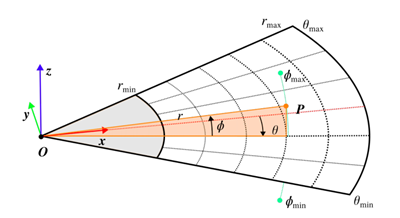
\includegraphics[width = 0.8\textwidth]{声纳成像1.png}
\caption{单个声纳图像的几何结构,点 $P$ 由范围 $r$、仰角 $\Phi$ 和方位角 $\theta$ 表示。\\
  $r_{\min}$, $r_{\max}$, $\Phi_{\min}$, $\Phi_{\max}$, $\theta_{\min}$, $\theta_{\max}$ 分别是成像声纳的最大和最小范围,\\
  最大仰角和最小仰角,最大方位角和最小方位角。}
\label{fig:声纳成像1}
\end{figure}

成像声纳通过发出一系列类似锥形的声波信号来生成部分球面测量值,从收发器测量观察到的反射信号的飞行时间,提供了反射表面的范围 $r$ 和方位角 $\theta$。但是这样的测量无法准确判断出
仰角 $\Phi$。因此,所有来自同一个方位角和距离的检测回波都会投影到声纳图像上的同一点 $I$( $\theta$, $r$),如图\ref{fig:声纳成像2}所示。对于对应于 $I$ 点中的某个方位角和距离
的像素,像素的强度对应于该方位角和距离下所有回波反射信号的强度。

\begin{figure}[ht]
	\centering
	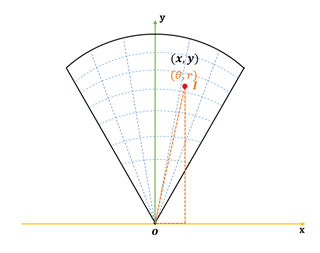
\includegraphics[width = 0.8\textwidth]{声纳成像2.png}
	\caption{真实声纳图像是整个垂直声纳数据在2D平面的投影。}
	\label{fig:声纳成像2}
\end{figure}

为了直观展示前视声纳的成像特征与其在水下环境感知中的应用,如图\ref{fig:水下机器人视觉图像与前视声纳图像对应示意图}所示,展示了同一时刻下水下机器人采集到的视觉图像与对应的前视
声纳图像。视觉图像反映了光学成像下的场景特征,可见由于水下光线传播的限制,视觉图像中的细节信息较为模糊。而前视声纳图像则通过声波反射捕捉了场景的结构信息,能够清晰地显示出障碍
物和地形特征。两者在信息维度和感知机制上存在显著差异。

需要指出的是,前视声纳图像通常可以以两种方式进行表示:一种是基于声纳测量参数,以方位角和距离为坐标轴的极坐标图像,直接对应于声纳的观测几何结构;另一种是通过坐标变换,
如公式\eqref{eq:coord}和\eqref{eq:polar}所示,


\begin{figure}[!ht]
	\centering
	% ---- 定义标准尺寸盒子(以第一张图为基准)----
	\newsavebox{\standardbox}
	\savebox{\standardbox}{%
	  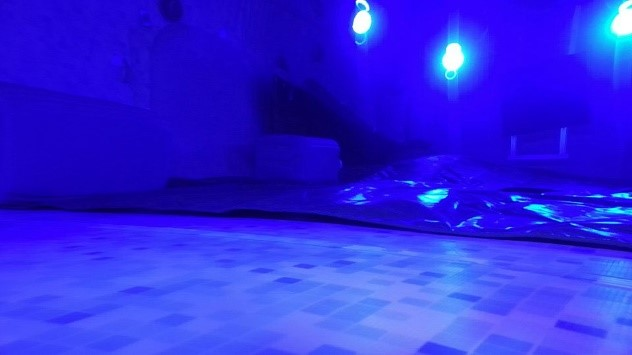
\includegraphics[width=0.47\textwidth]{figures/2-2视觉图像.jpg}%
	}
  
	% ---- 两张图并排,强制等宽等高 ----
	\begin{minipage}{\textwidth}
	  \centering
	  \subfigure[视觉图像\label{fig:2-2视觉图像}]{%
		\usebox{\standardbox}% 第一张:原始尺寸
	  }\hspace{1em}
	  \subfigure[前视声纳图像\label{fig:2-2声纳图像}]{%
		\resizebox{!}{\ht\standardbox}{% 强制等高
		  \resizebox{\wd\standardbox}{!}{% 强制等宽
			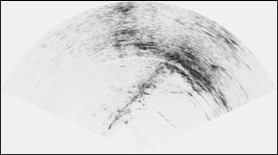
\includegraphics{figures/2-2声纳图像.jpg}%
		  }%
		}%
	  }
	\end{minipage}
  
	\caption{水下机器人视觉图像与前视声纳图像对应示意图}
	\label{fig:水下机器人视觉图像与前视声纳图像对应示意图}
  \end{figure}



\subsection{并排图和子图}[Abreast-picture and Sub-picture example]
\subsubsection{并排图}[Abreast-picture example]

使用并排图时,需要注意对齐方式。默认情况是中部对齐。这里给出中部对齐、顶部对齐
、图片底部对齐三种常见方式。其中,底部对齐方式有一个很巧妙的方式,将长度比较小
的图放在左面即可。

\lipsum[2]

\begin{figure}[htbp]
\centering
\begin{minipage}{0.4\textwidth}
\centering
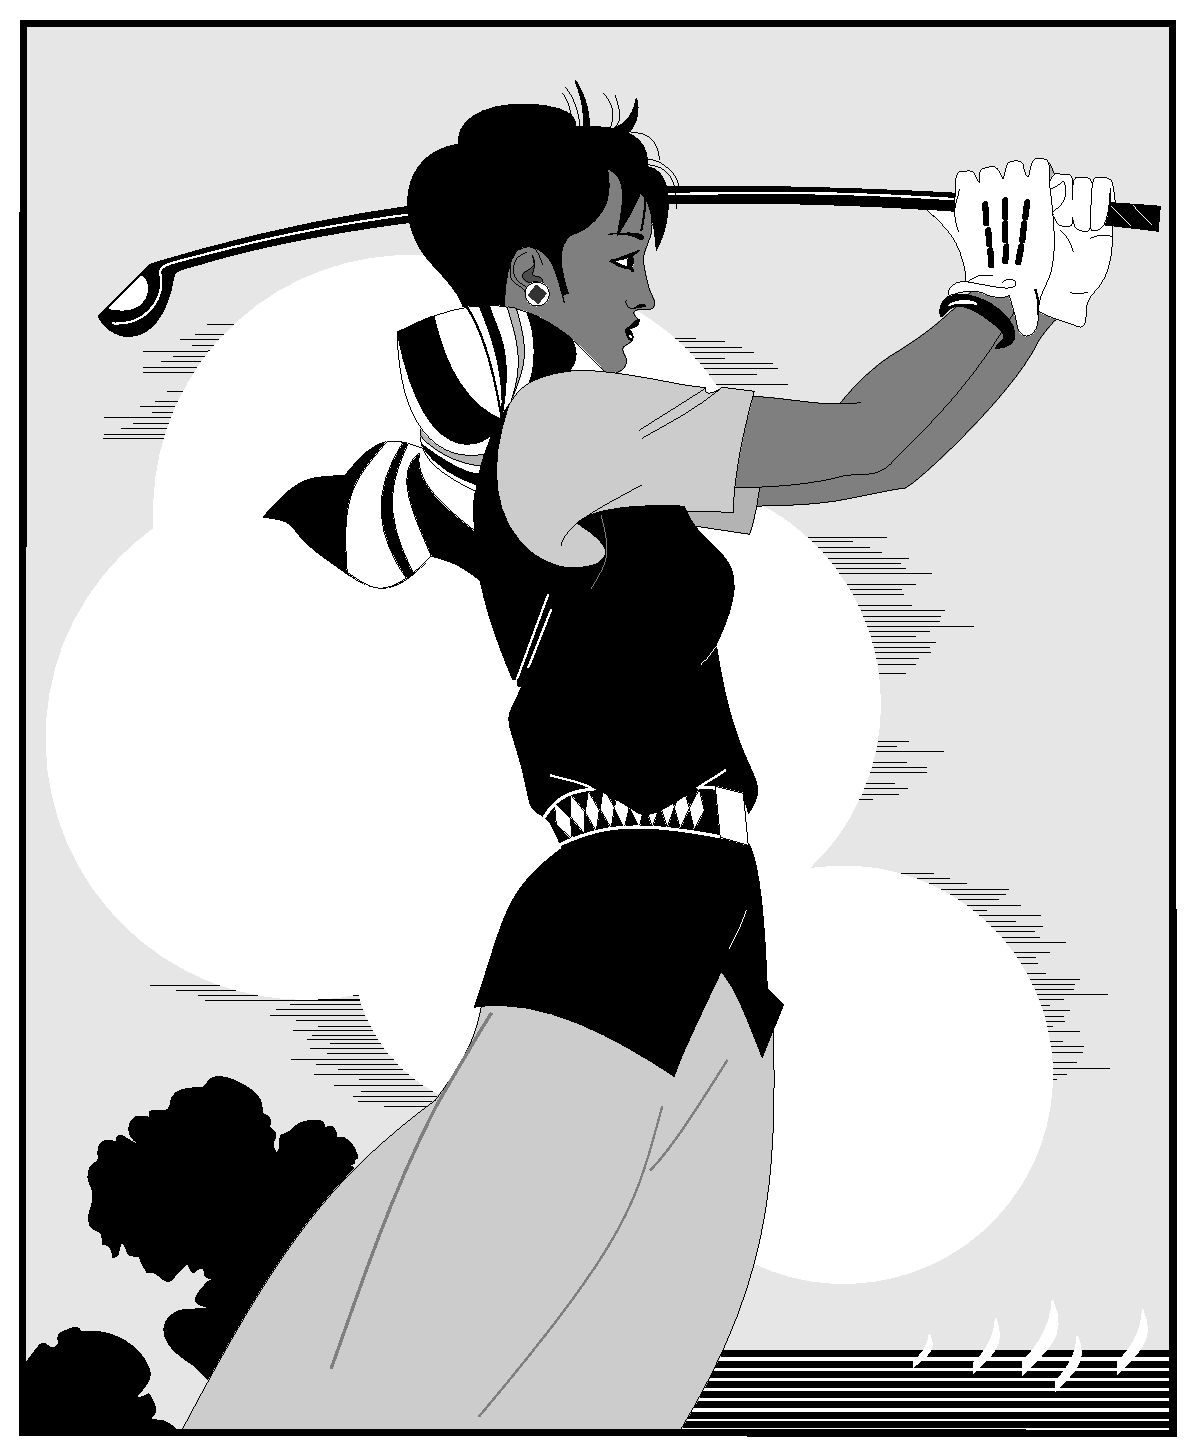
\includegraphics[width=\textwidth]{golfer}
\bicaption[golfer2]{}{打高尔夫球的人}{Fig.$\!$}{The person playing golf}
\end{minipage}
\centering
\begin{minipage}{0.4\textwidth}
\centering
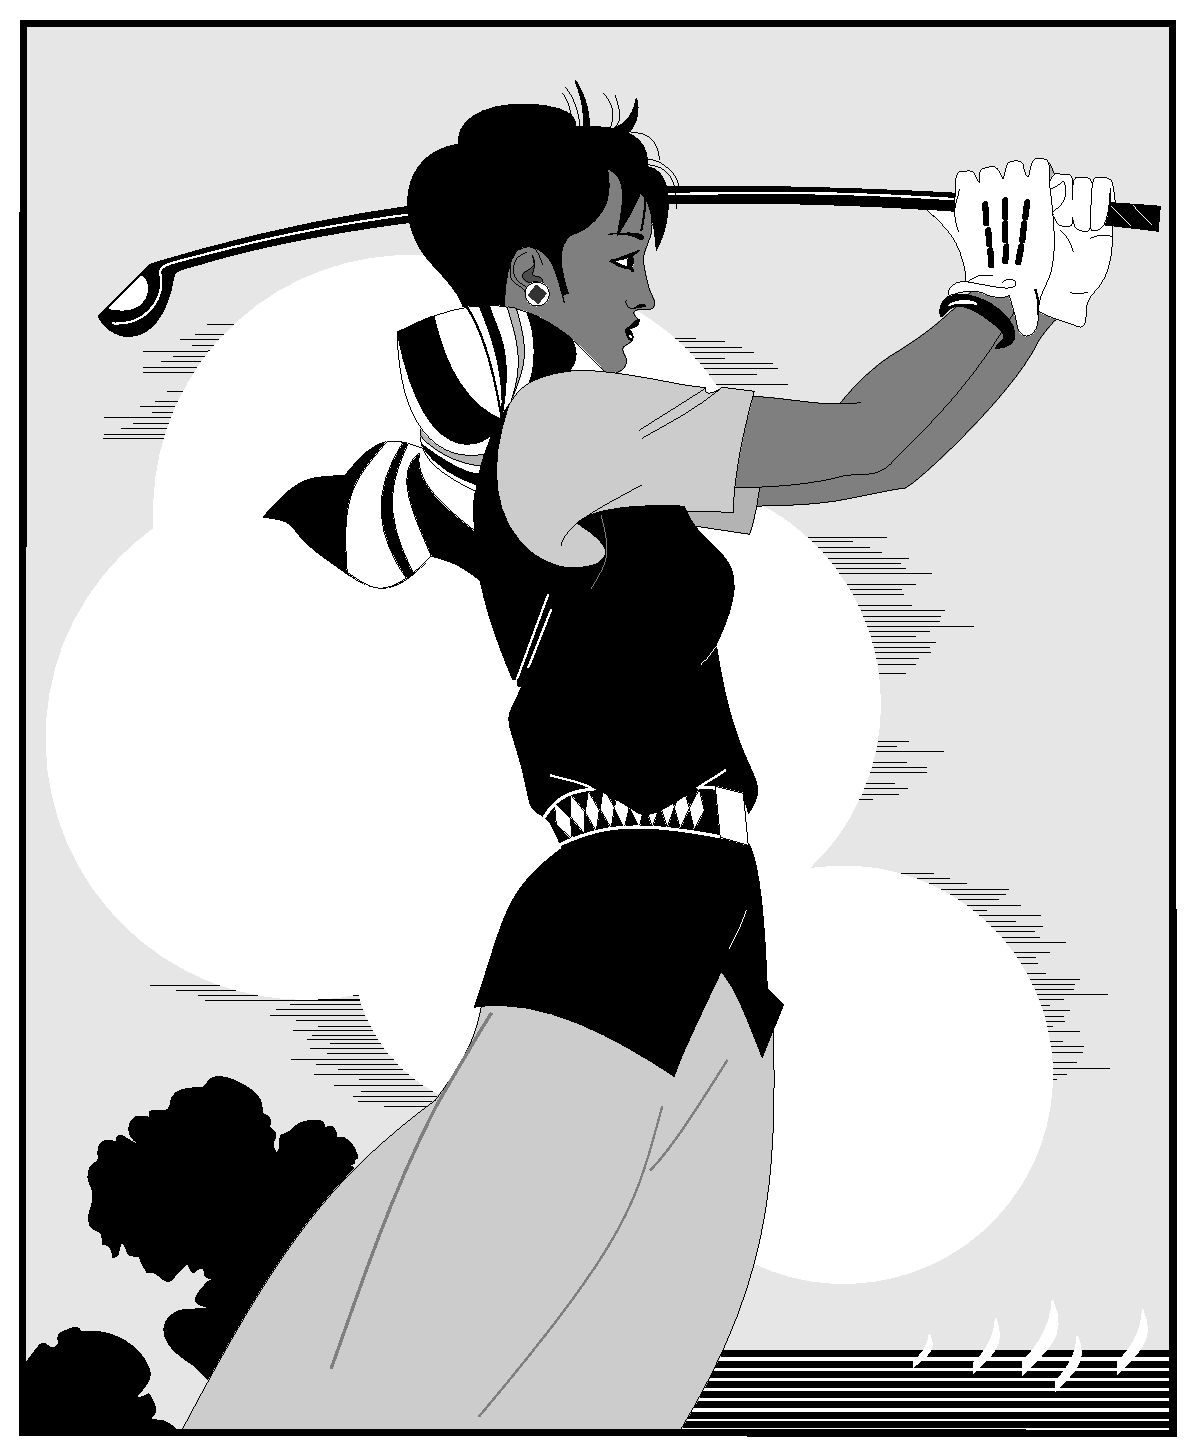
\includegraphics[width=\textwidth]{golfer}
\bicaption[golfer3]{}{打高尔夫球的人。注意,这里默认居中}{Fig.$\!$}{The person playing golf. Please note that, it is vertically center aligned by default.}
\end{minipage}
\end{figure}

\begin{figure}[htbp]
\centering
\begin{minipage}[t]{0.4\textwidth}
\centering
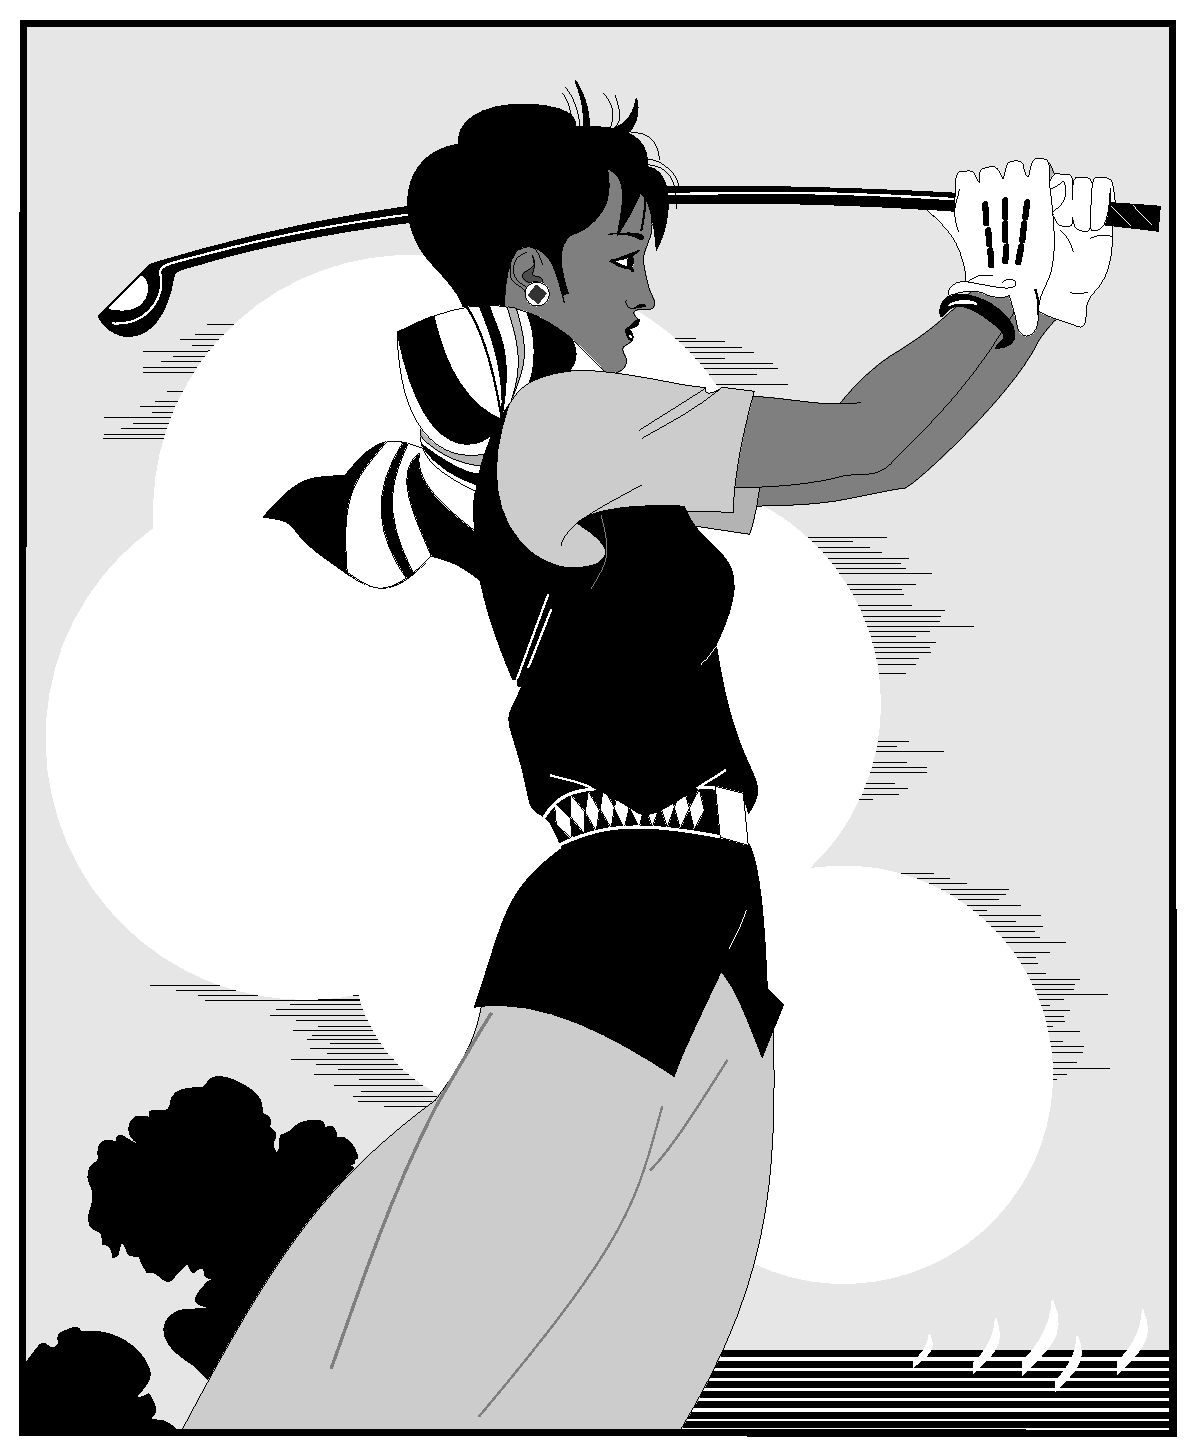
\includegraphics[width=\textwidth]{golfer}
\bicaption[golfer5]{}{打高尔夫球的人}{Fig.$\!$}{The person playing golf}
\end{minipage}
\centering
\begin{minipage}[t]{0.4\textwidth}
\centering
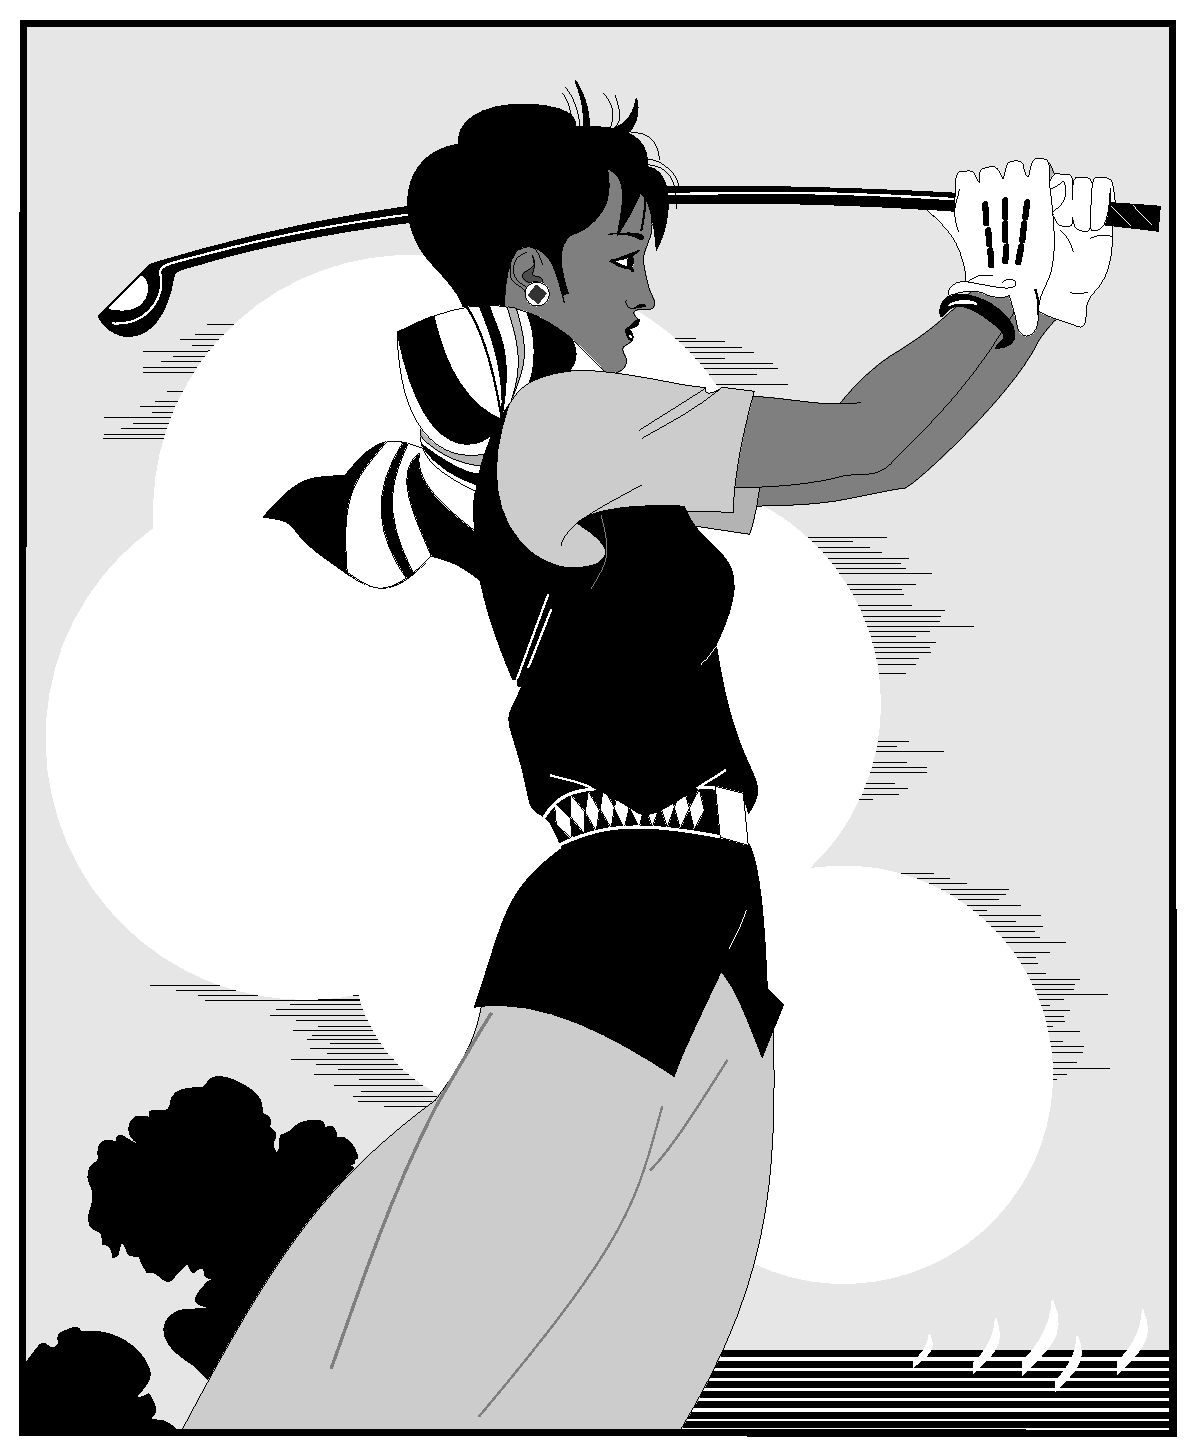
\includegraphics[width=\textwidth]{golfer}
\bicaption[golfer8]{}{打高尔夫球的人。注意,此图是顶部对齐}{Fig.$\!$}{The person playing golf. Please note that, it is vertically top aligned.}
\end{minipage}
\end{figure}

\begin{figure}[htbp]
\centering
\begin{minipage}[t]{0.4\textwidth}
\centering
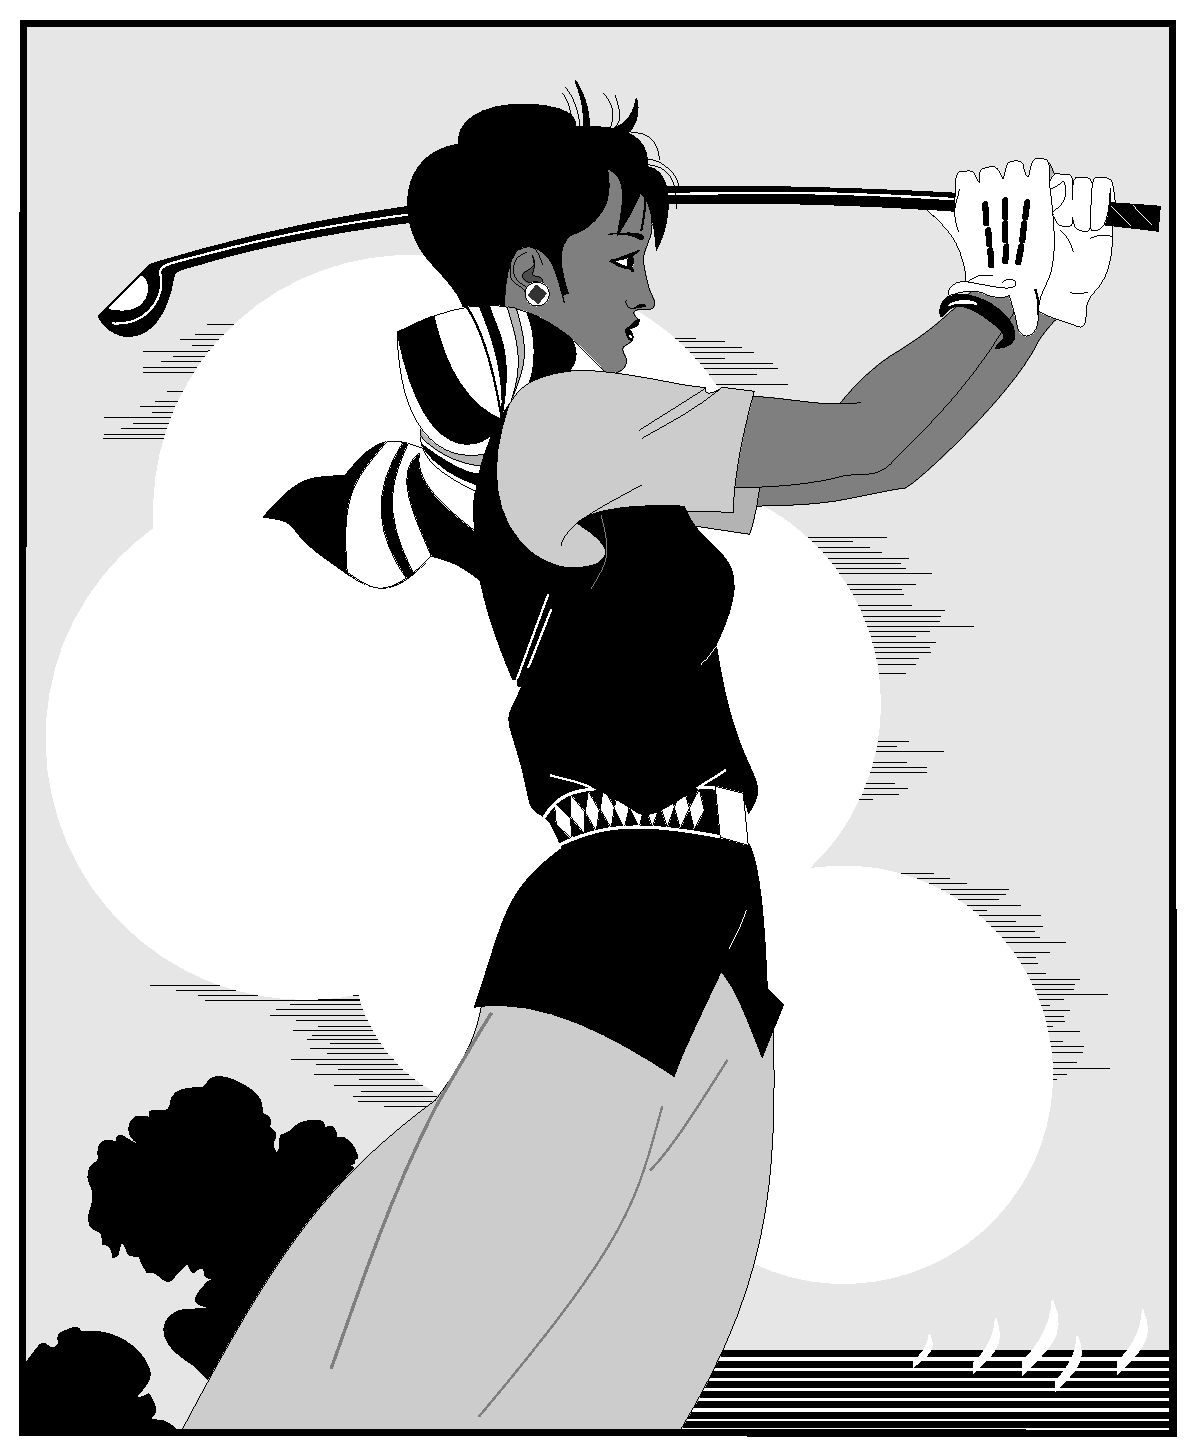
\includegraphics[width=\textwidth,height=\textwidth]{golfer}
\bicaption[golfer9]{}{打高尔夫球的人。注意,此图对齐方式是图片底部对齐}{Fig.$\!$}{The person playing golf. Please note that, it is vertically bottom aligned for figure.}
\end{minipage}
\centering
\begin{minipage}[t]{0.4\textwidth}
\centering
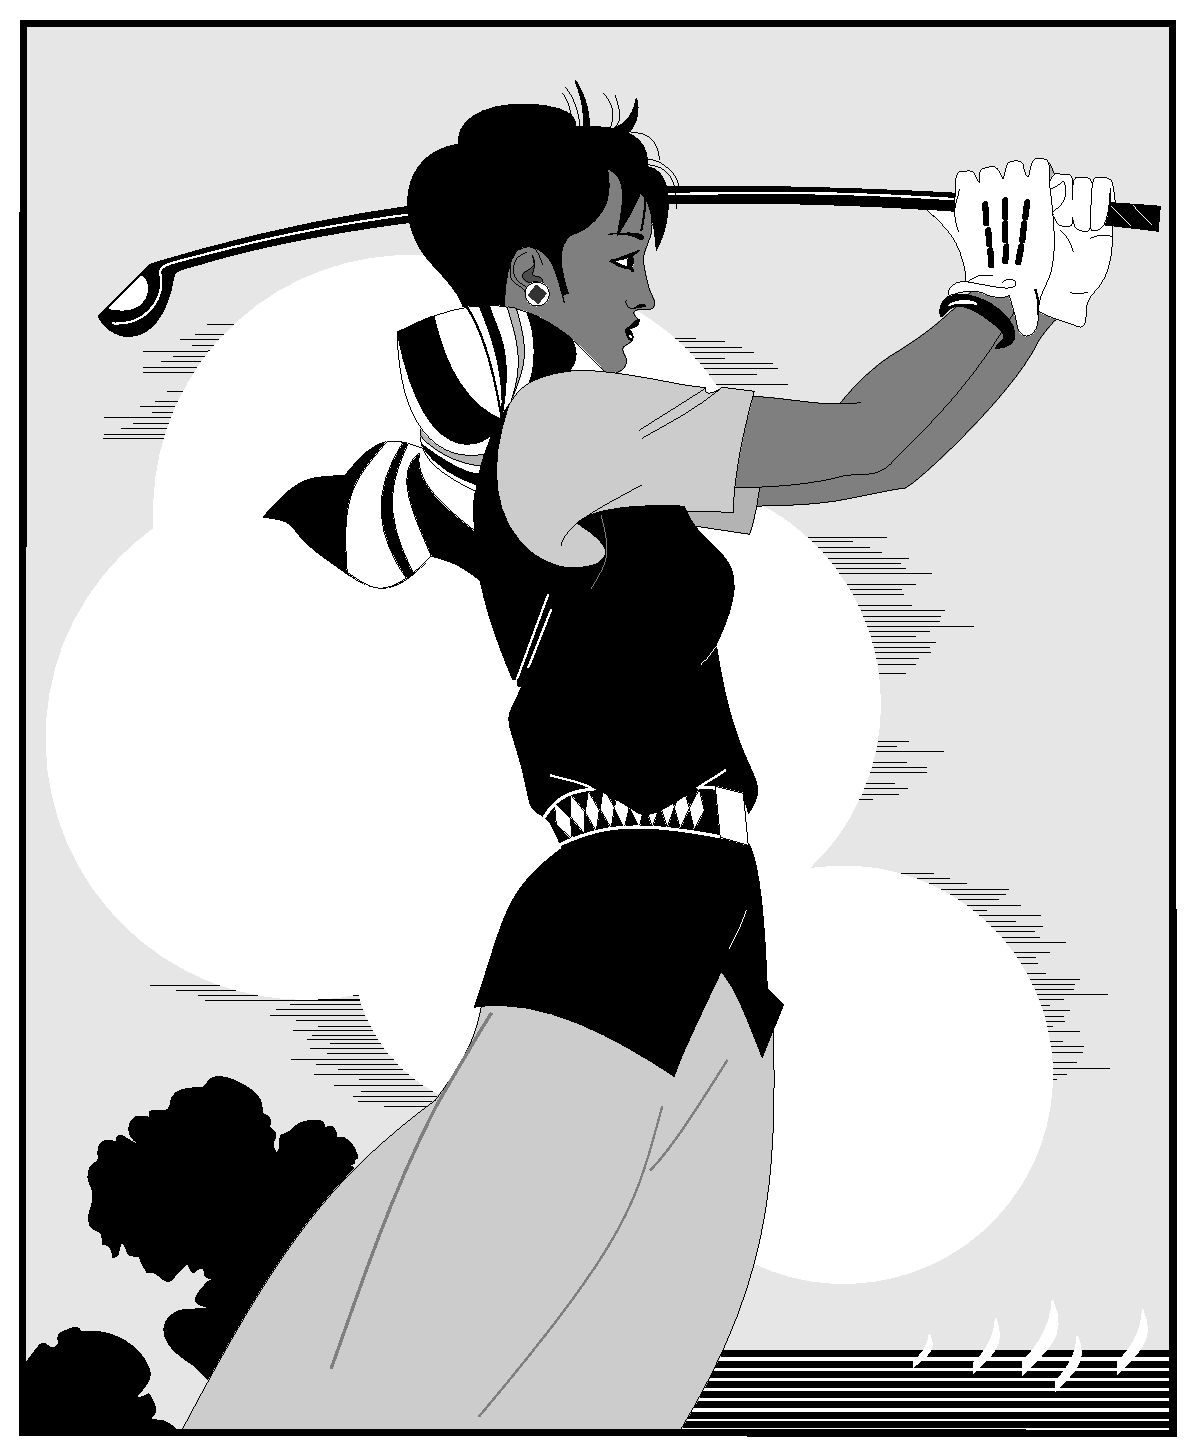
\includegraphics[width=\textwidth]{golfer}
\bicaption[golfer6]{}{打高尔夫球的人}{Fig.$\!$}{The person playing golf}
\end{minipage}
\end{figure}

\subsubsection{子图}[Sub-picture example]

注意:子图题注也可以只用中文。规范规定“分图题置于分图之下或图题之下”,但没有给出具体的格式要求。
没有要求的另外一个说法就是“无论什么格式都不对”。
所以只有在一个图中有标注“(a),(b)”,无法使用\cs{subfigure}的情况下,使用最后一个图例中的格式设置方法,否则不要使用。
为了应对“无论什么格式都不对”,这个子图图题使用“minipage”和“description”环境,宽度,对齐方式可以按照个人喜好自由设置,是否使用双语子图图题也可以自由设置。

\lipsum[1-3]

无意义文字,每页底部不要留空白。

\lipsum[4-5]

\begin{figure}[!ht]
\setlength{\subfigcapskip}{-1bp}
\centering
\begin{minipage}{\textwidth}
\centering
\subfigure{\label{golfer41}}\addtocounter{subfigure}{-2}
\subfigure[The person playing golf]{\subfigure[打高尔夫球的人~1]{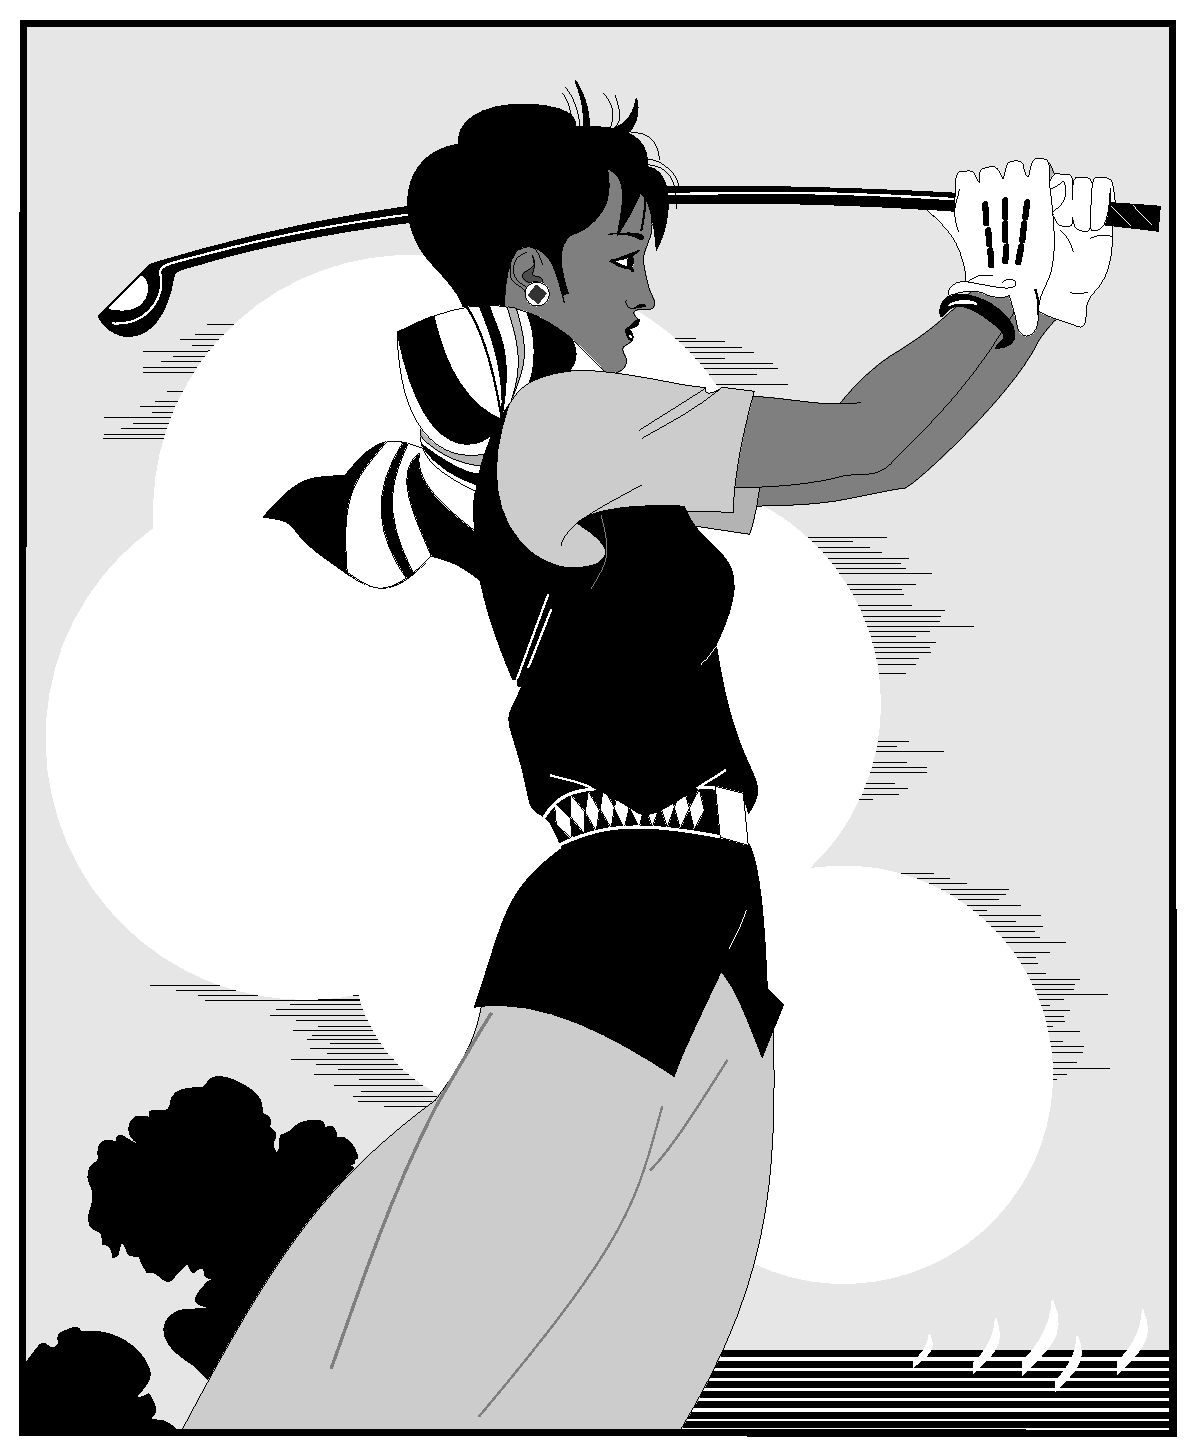
\includegraphics[width=0.4\textwidth]{golfer}}}
\hspace{2em}
\subfigure{\label{golfer42}}\addtocounter{subfigure}{-2}
\subfigure[The person playing golf]{\subfigure[打高尔夫球的人~2]{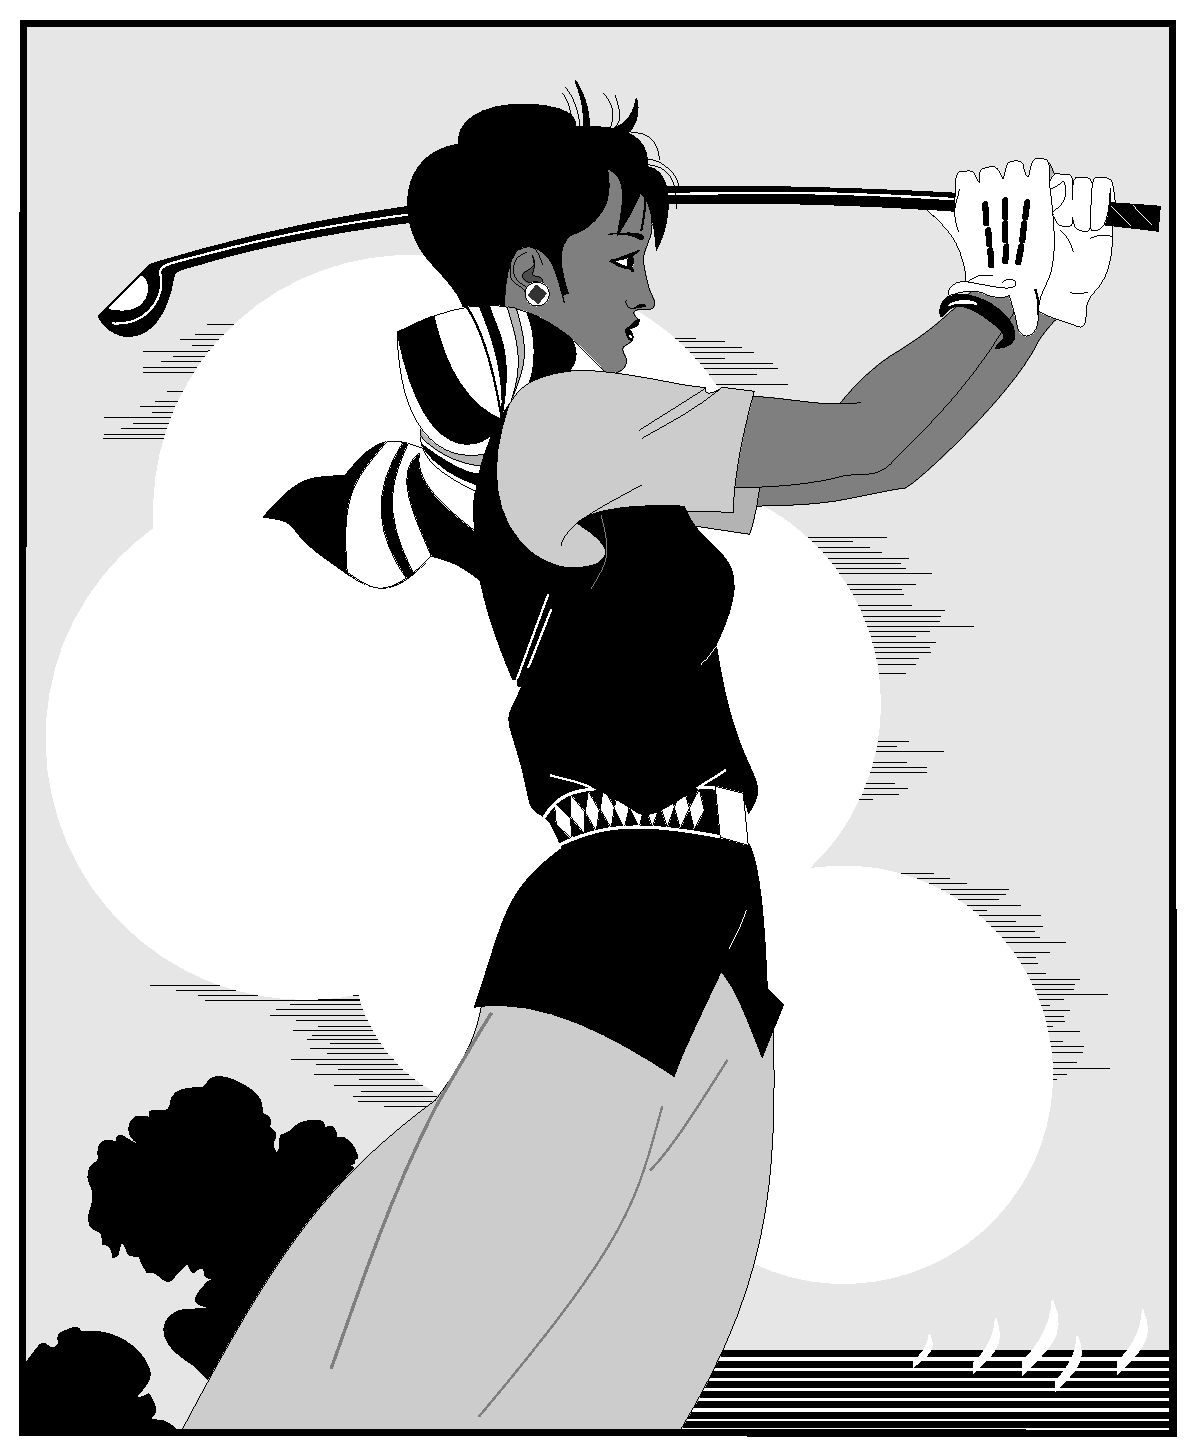
\includegraphics[width=0.4\textwidth]{golfer}}}
\end{minipage}
\centering
\begin{minipage}{\textwidth}
\centering
\subfigure{\label{golfer43}}\addtocounter{subfigure}{-2}
\subfigure[The person playing golf]{\subfigure[打高尔夫球的人~3]{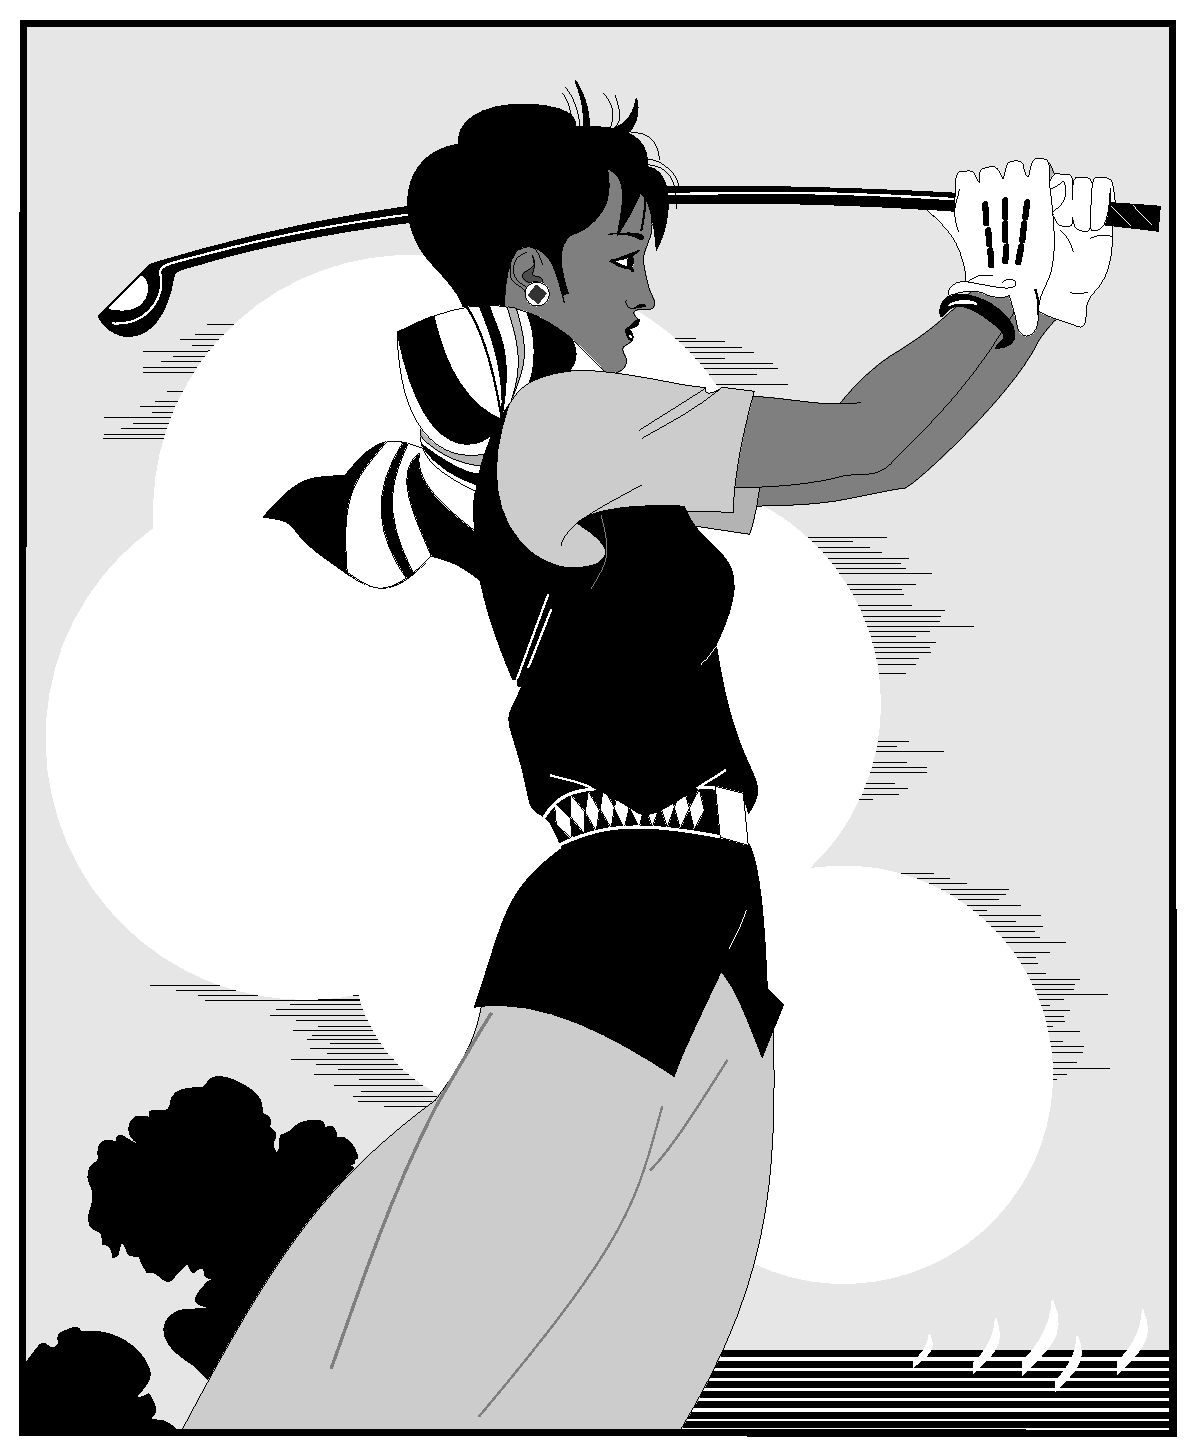
\includegraphics[width=0.4\textwidth]{golfer}}}
\hspace{2em}
\subfigure{\label{golfer44}}\addtocounter{subfigure}{-2}
\subfigure[The person playing golf. Here, 'hang indent' and 'center last line' are not stipulated in the regulation.]{\subfigure[打高尔夫球的人~4。注意,规范中没有明确规定要悬挂缩进、最后一行居中。]{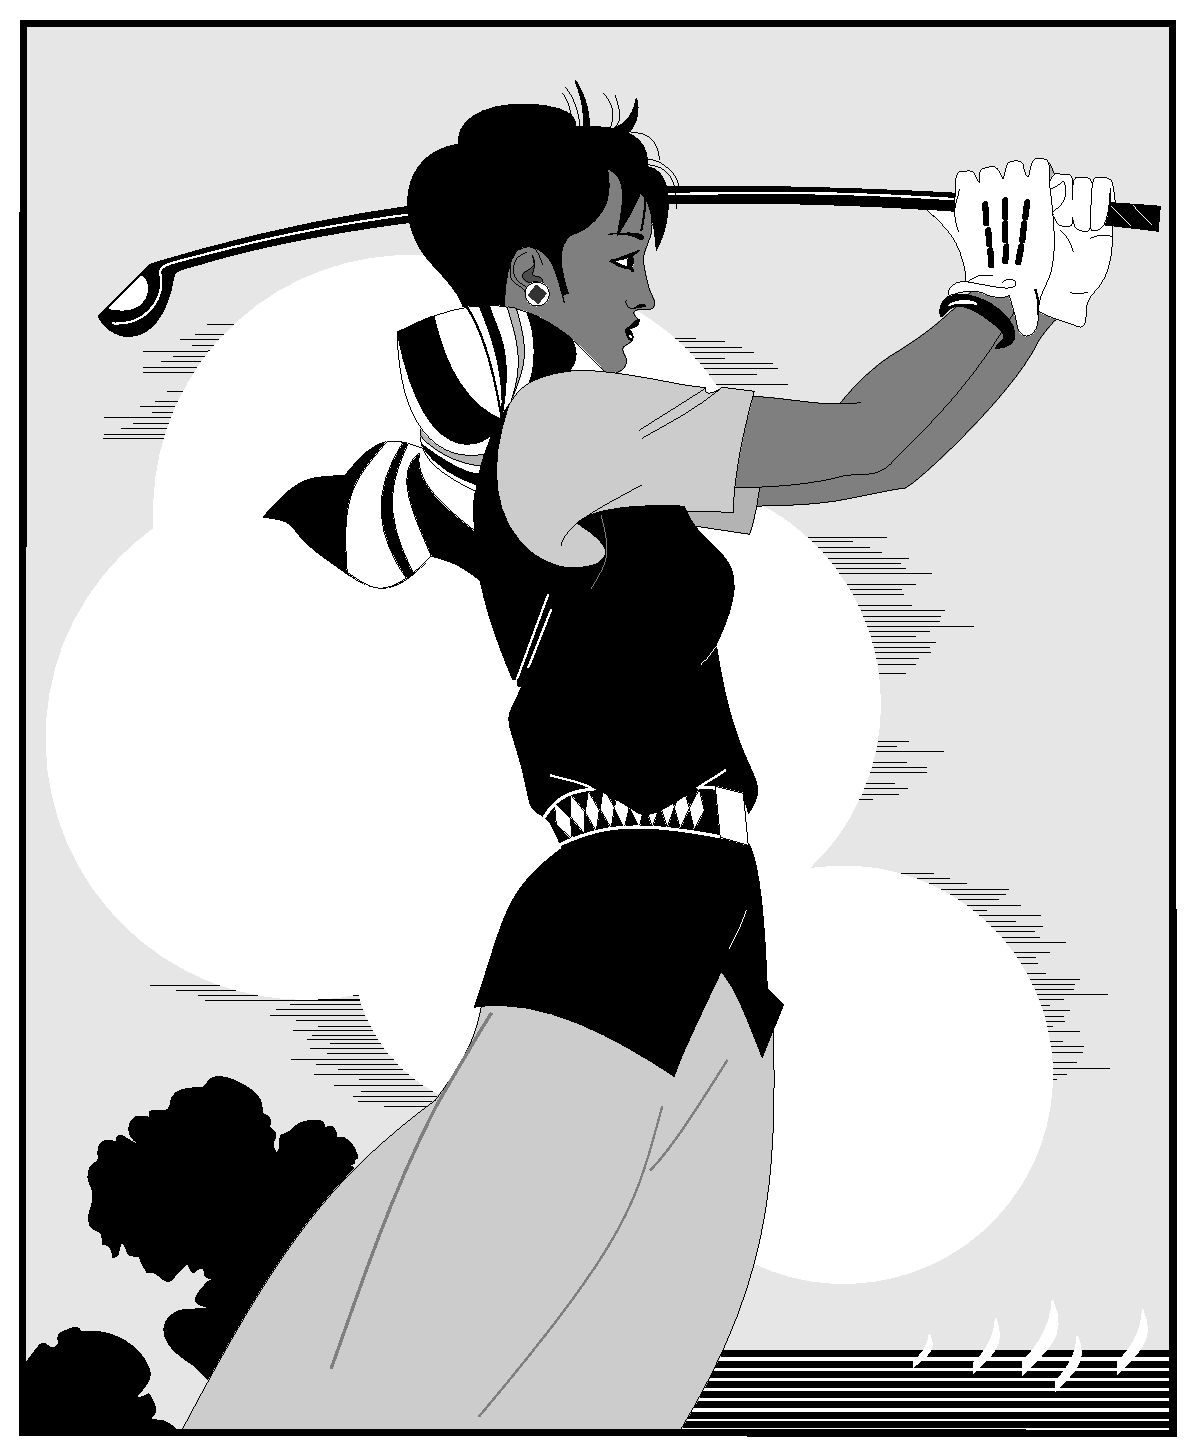
\includegraphics[width=0.4\textwidth]{golfer}}}
\end{minipage}
\vspace{0.2em}
\bicaption[golfer4]{}{打高尔夫球的人}{Fig.$\!$}{The person playing gol}
\end{figure}

\begin{figure}[t]
  \centering
  \begin{minipage}{.7\linewidth}
    \setlength{\subfigcapskip}{-1bp}
    \centering
    \begin{minipage}{\textwidth}
      \centering
      \subfigure{\label{golfer45}}\addtocounter{subfigure}{-2}
      \subfigure[The person playing golf]{\subfigure[打高尔夫球的人~1]{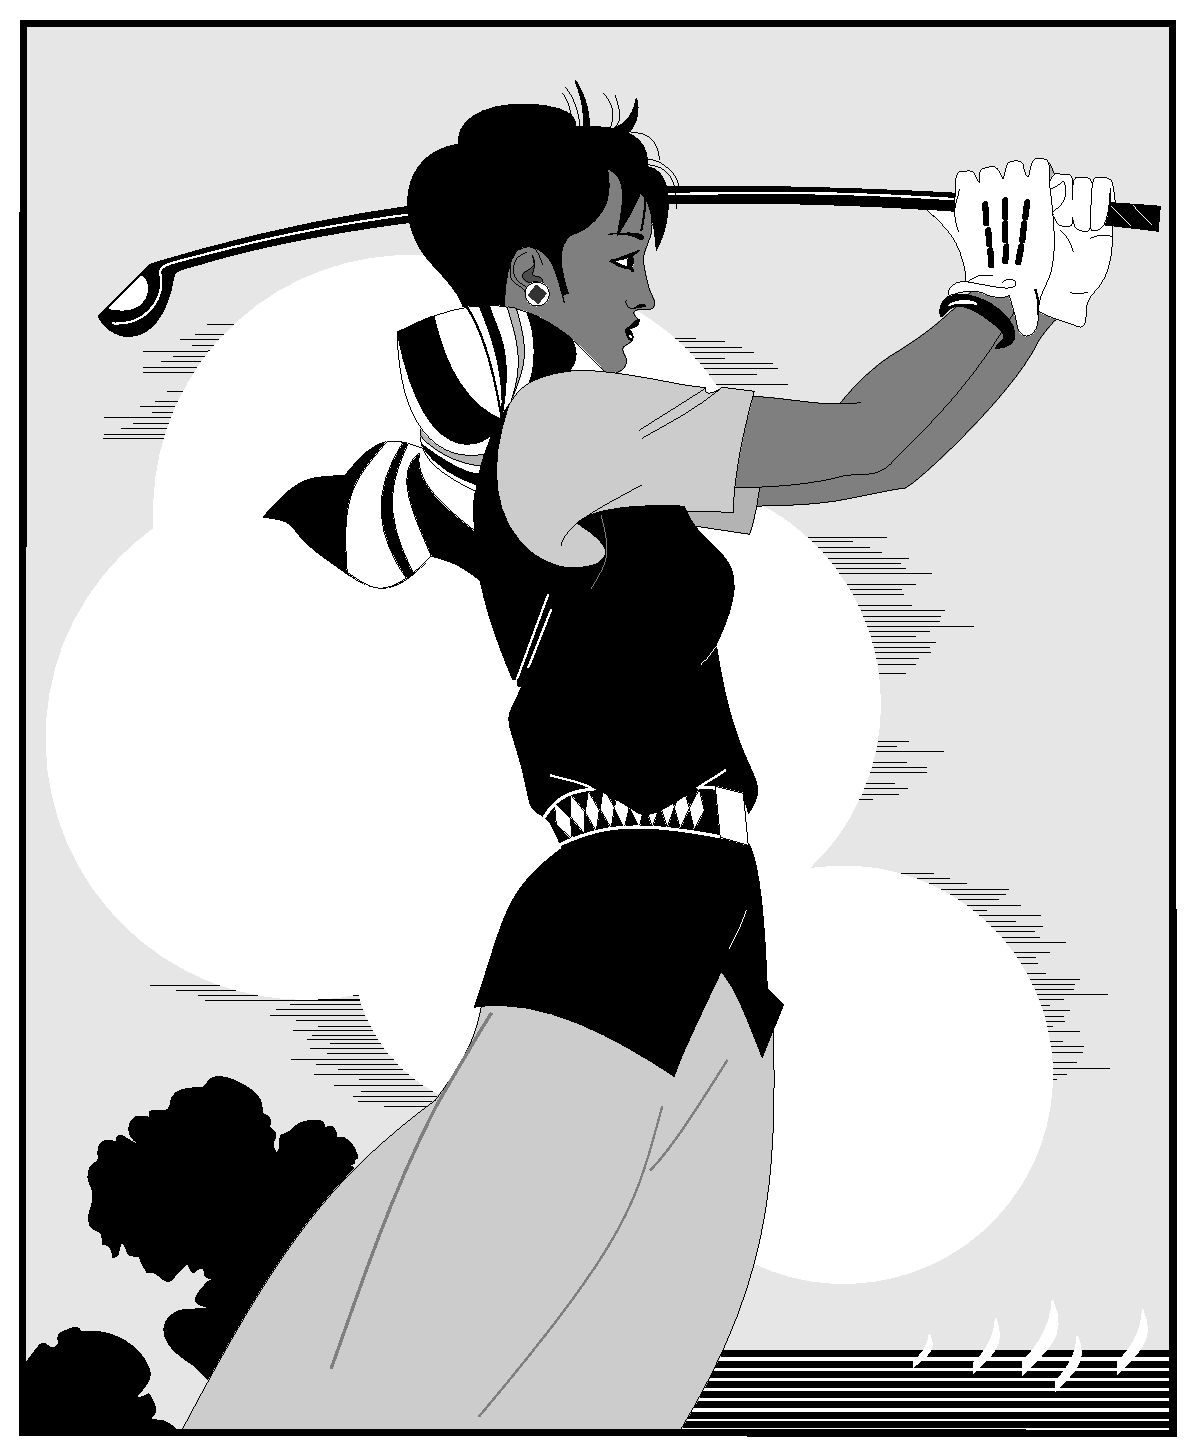
\includegraphics[width=0.4\textwidth]{golfer}}}
      \hspace{4em}
      \subfigure{\label{golfer46}}\addtocounter{subfigure}{-2}
      \subfigure[The person playing golf]{\subfigure[打高尔夫球的人~2]{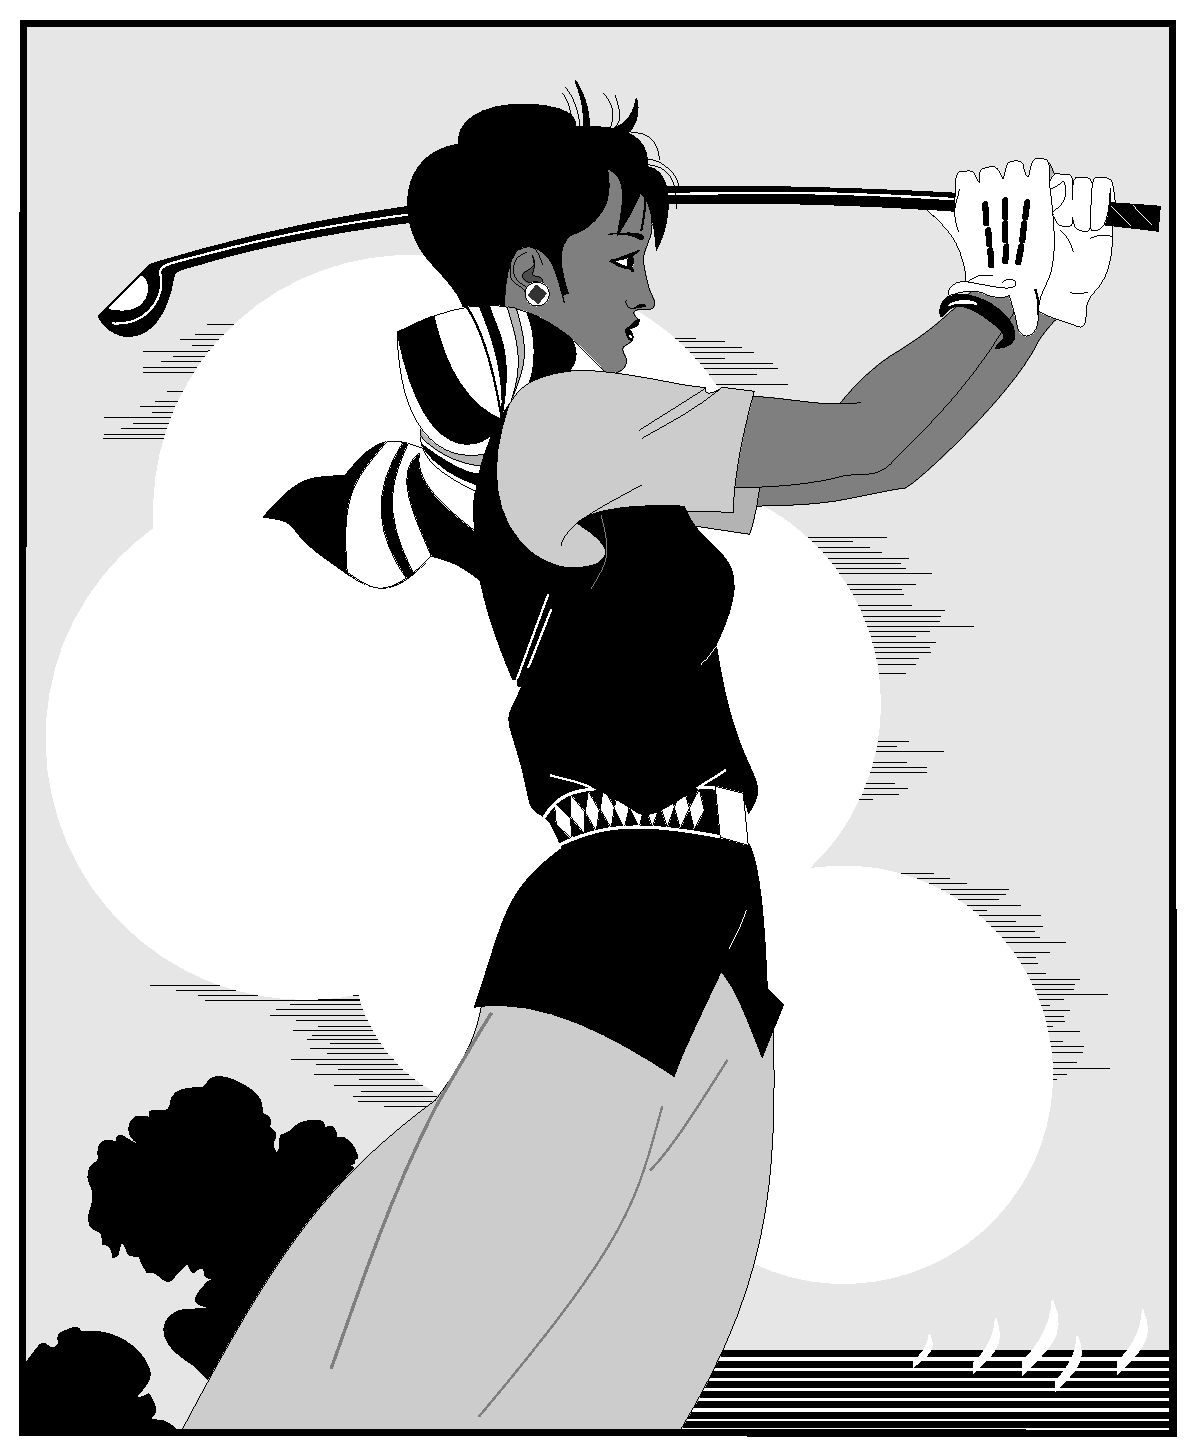
\includegraphics[width=0.4\textwidth]{golfer}}}
    \end{minipage}
    \vskip 0.2em
  \wuhao 注意:这里是中文图注添加位置(我工要求,图注在图题之上)。
    \vspace{0.2em}
\bicaption[golfer47]{}{打高尔夫球的人。注意,此处我工有另外一处要求,子图图题可以位于主图题之下。但由于没有明确说明位于下方具体是什么格式,所以这里不给出举例。}{Fig.$\!$}{The person playing golf. Please note that, although it is appropriate to put subfigures' captions under this caption as stipulated in regulation, but its format is not clearly stated.}
  \end{minipage}
\end{figure}

\begin{figure}[t]
\centering
% \begin{tikzpicture}
% 	\node[anchor=south west,inner sep=0] (image) at (0,0) {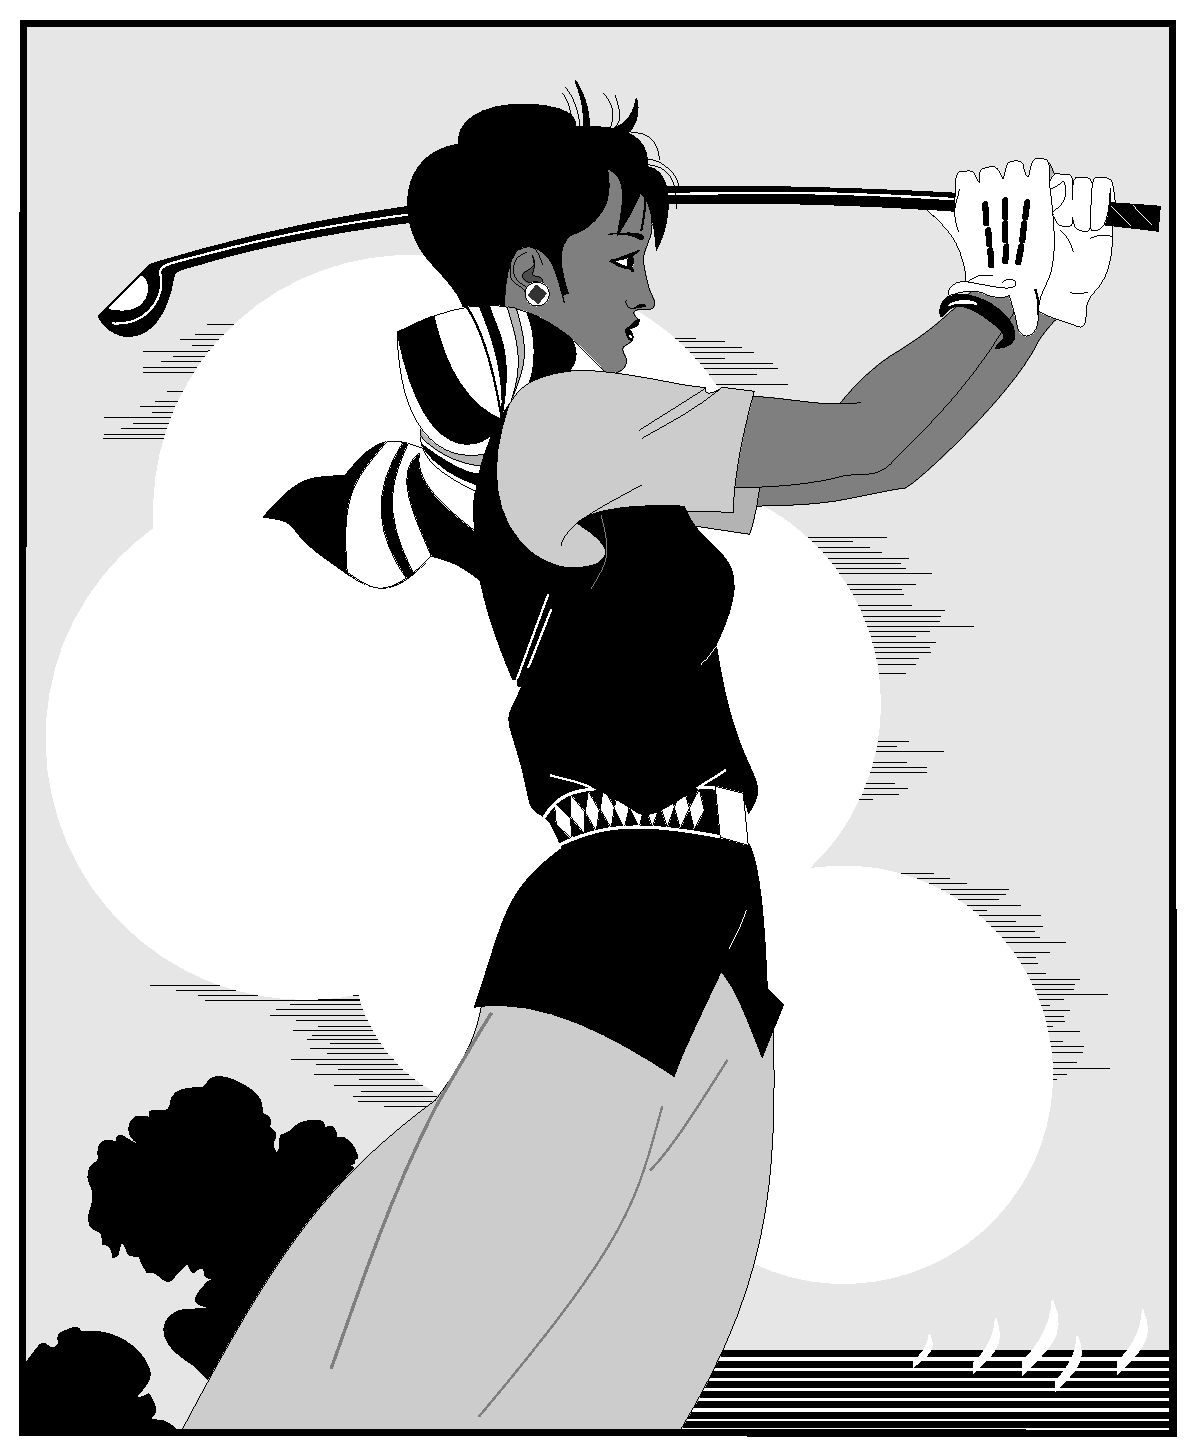
\includegraphics[width=0.3\textwidth]{golfer}};
% 	\begin{scope}[x={(image.south east)},y={(image.north west)}]
% 		\node at (0.3,0.5) {a)};
% 		\node at (0.8,0.2) {b)};
% 	\end{scope}
% \end{tikzpicture}
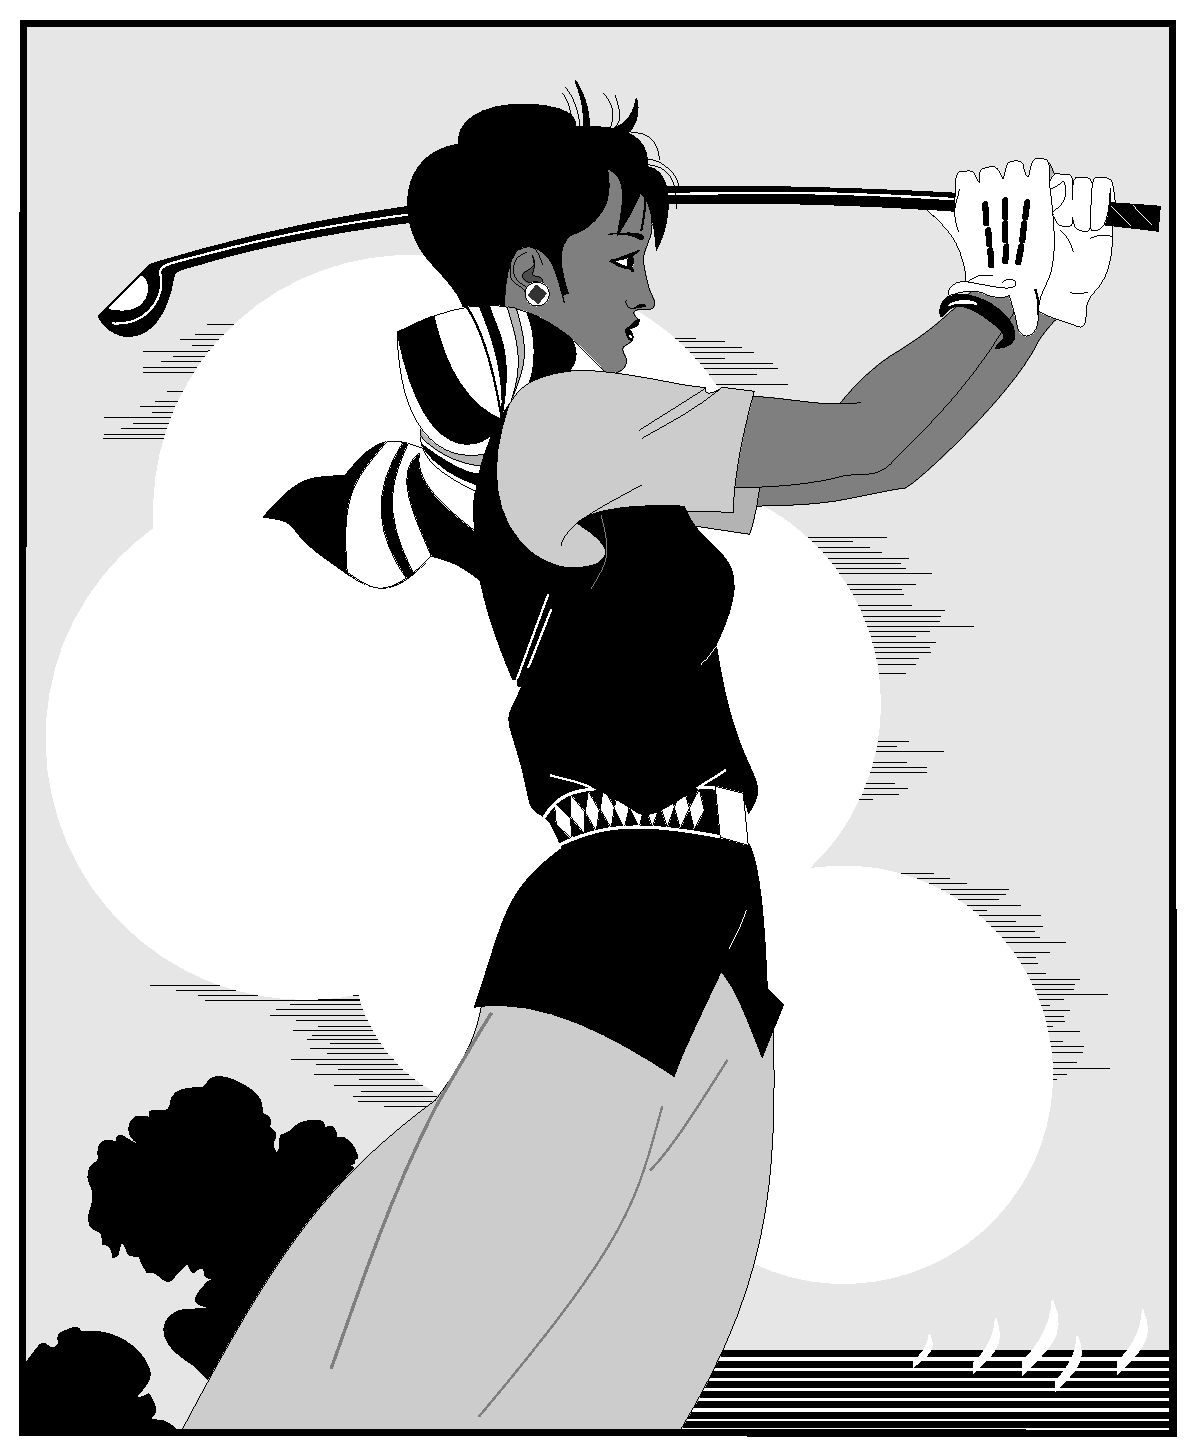
\includegraphics[width=0.3\textwidth]{golfer}
\bicaption[golfer0]{}{打高尔夫球球的人(博士论文双语题注)}{Fig.$\!$}{The person playing golf (Doctoral thesis)}
\vskip -0.4em
 \hspace{2em}
\begin{minipage}[t]{0.3\textwidth}
\wuhao \setlist[description]{font=\normalfont}
	\begin{description}
		\item[(a)]子图图题
		\item[(a)]Subfigure caption
	\end{description}
 \end{minipage}
 \hspace{2em}
 \begin{minipage}[t]{0.3\textwidth}
\wuhao \setlist[description]{font=\normalfont}
	\begin{description}
		\item[(b)]子图图题
		\item[(b)]Subfigure caption
	\end{description}
\end{minipage}
\end{figure}

\begin{figure}[!ht]
	\centering
	\begin{sideways}
		\begin{minipage}{\textheight}
			\centering
			\fbox{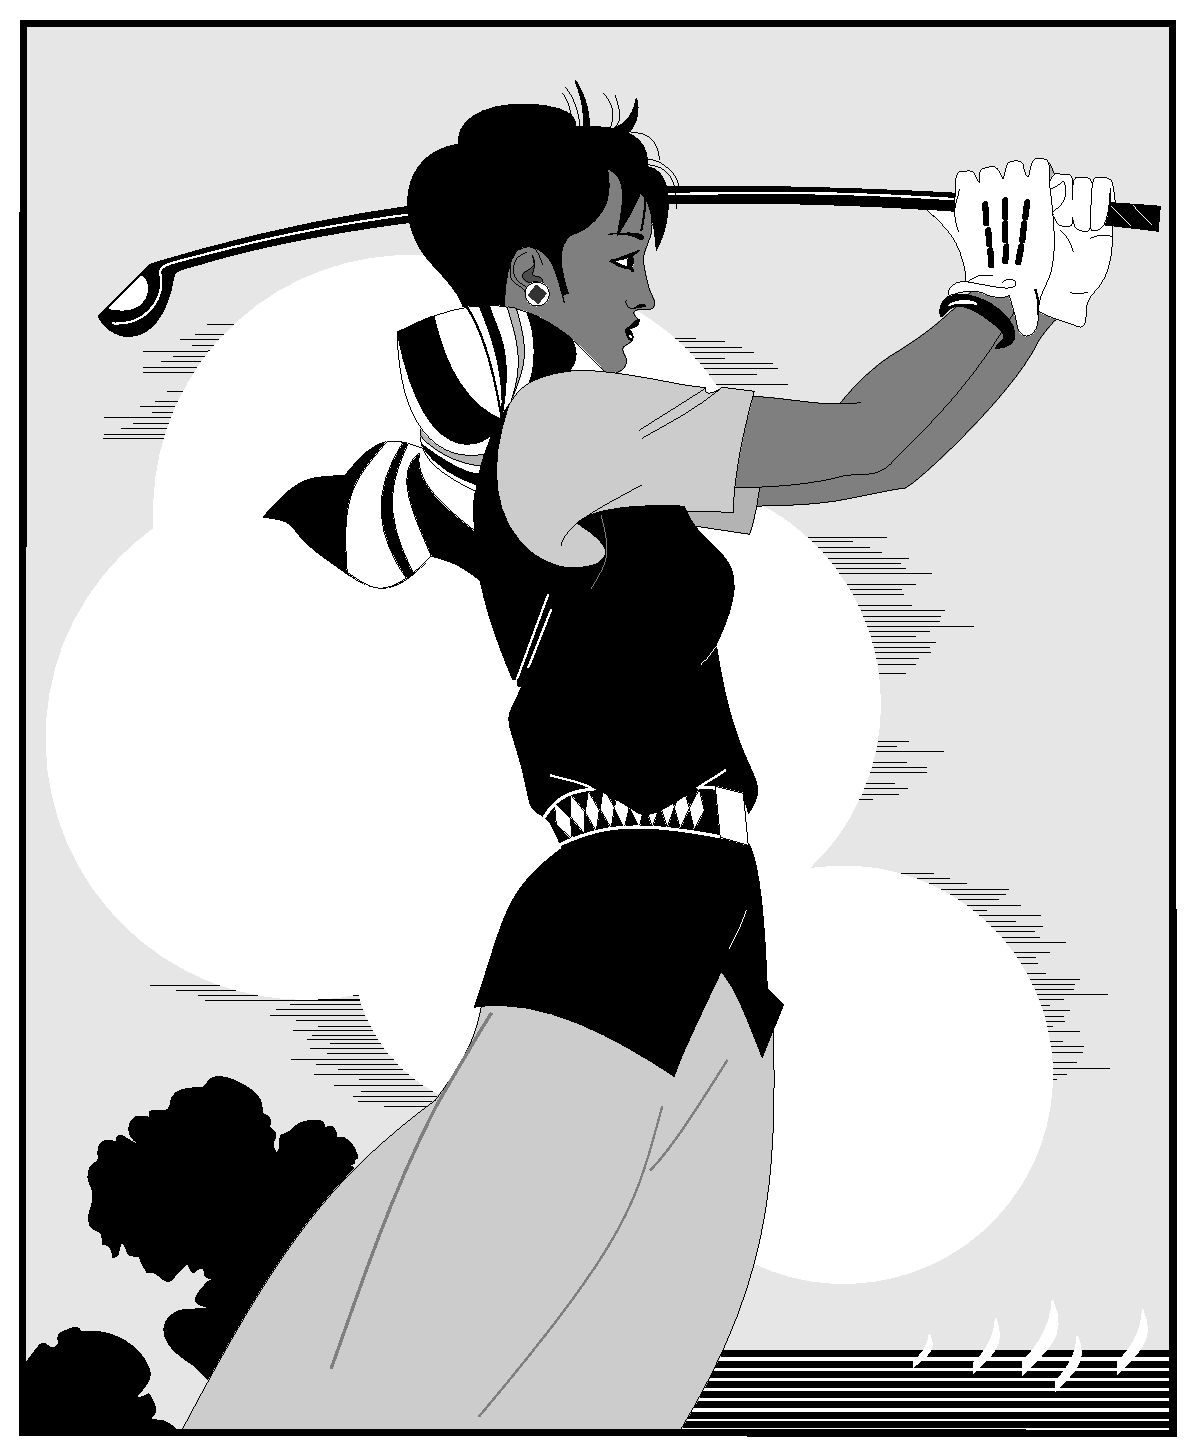
\includegraphics[width=0.2\textwidth]{golfer}}
			\fbox{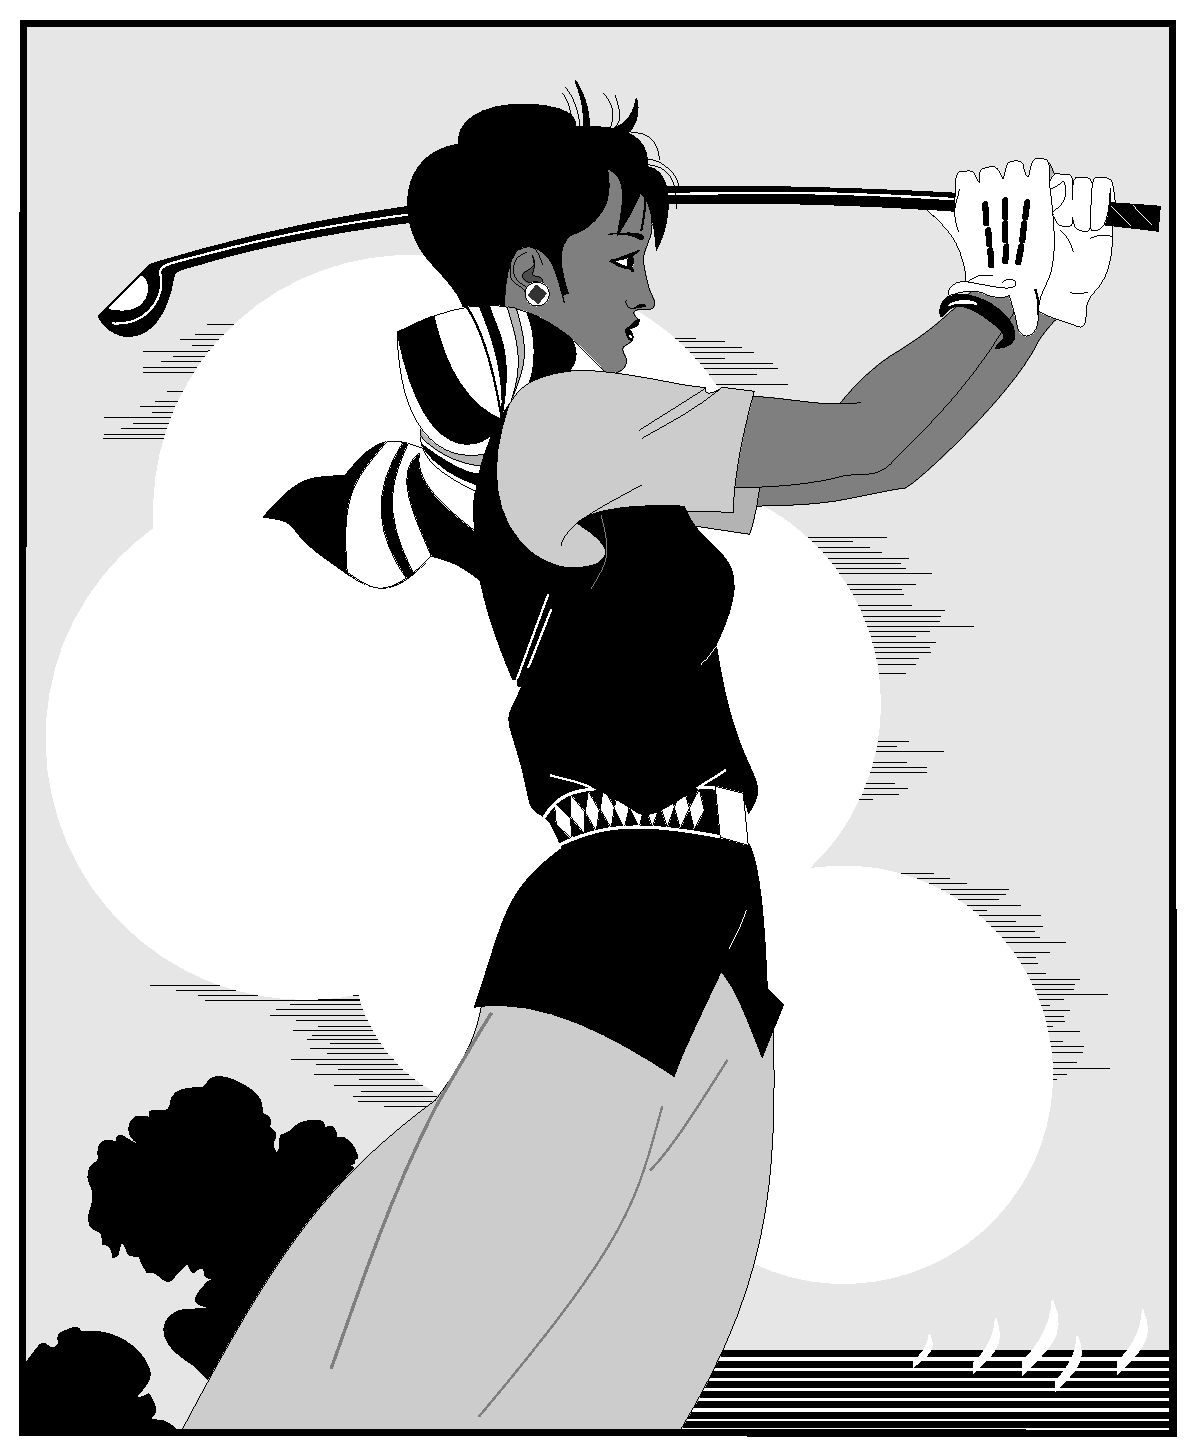
\includegraphics[width=0.2\textwidth]{golfer}}
			\fbox{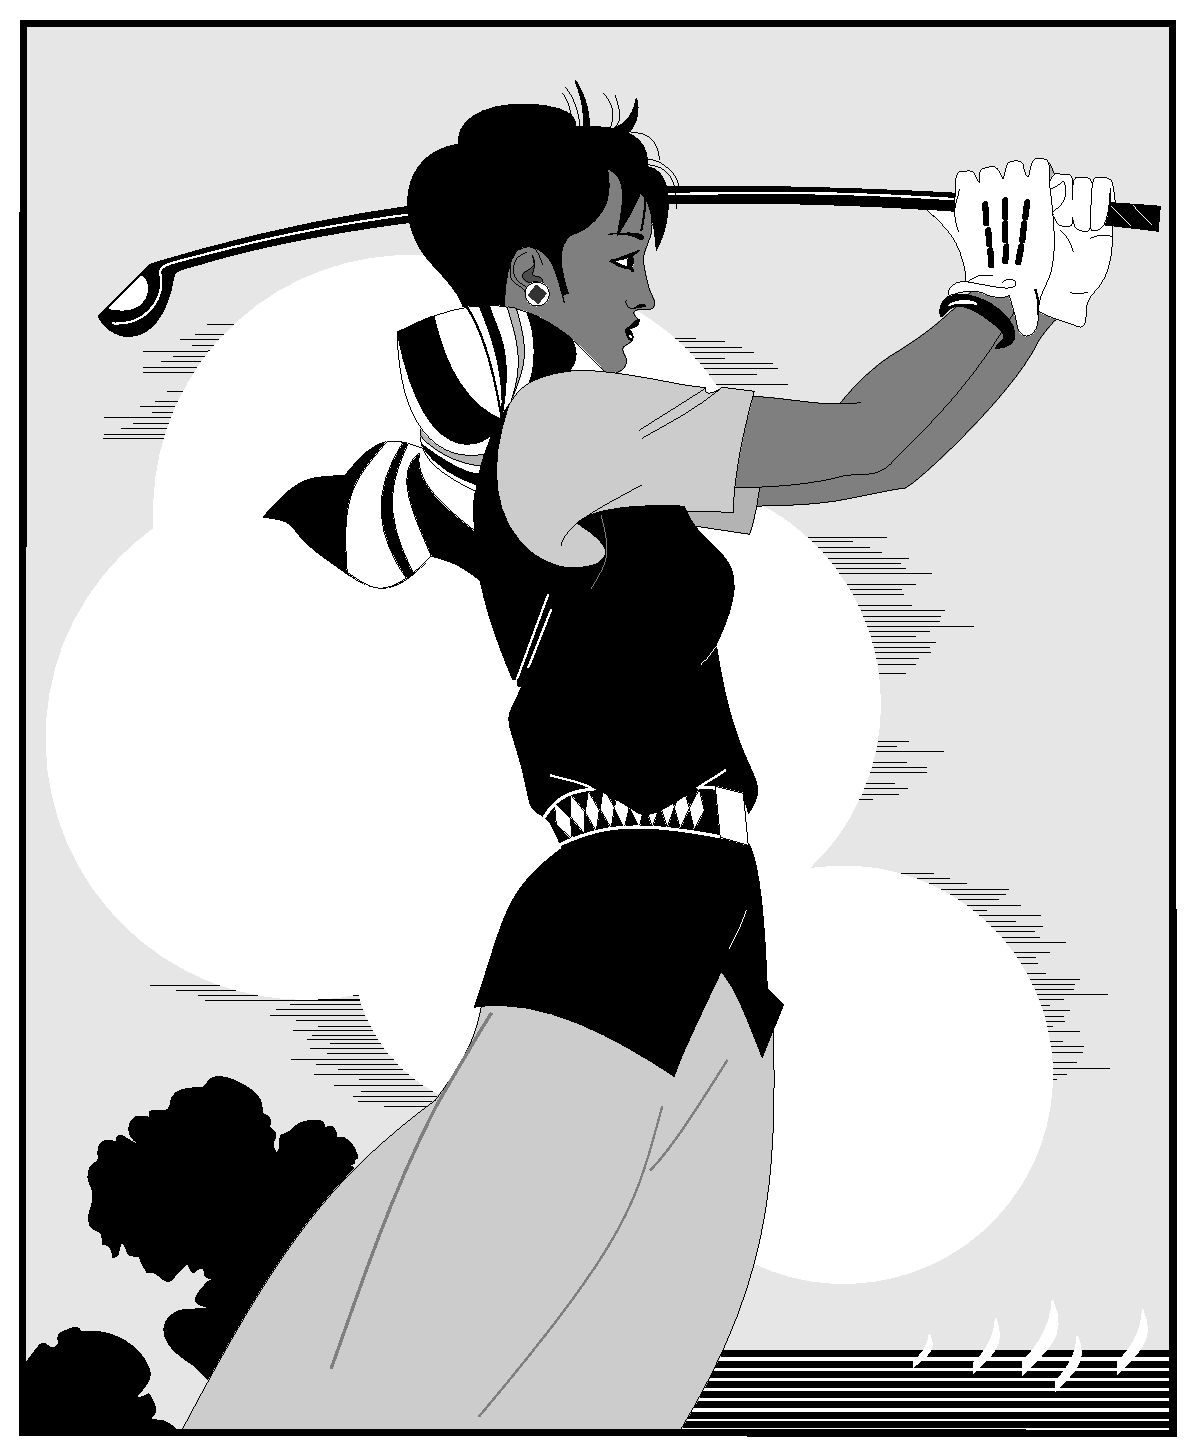
\includegraphics[width=0.2\textwidth]{golfer}}
			\fbox{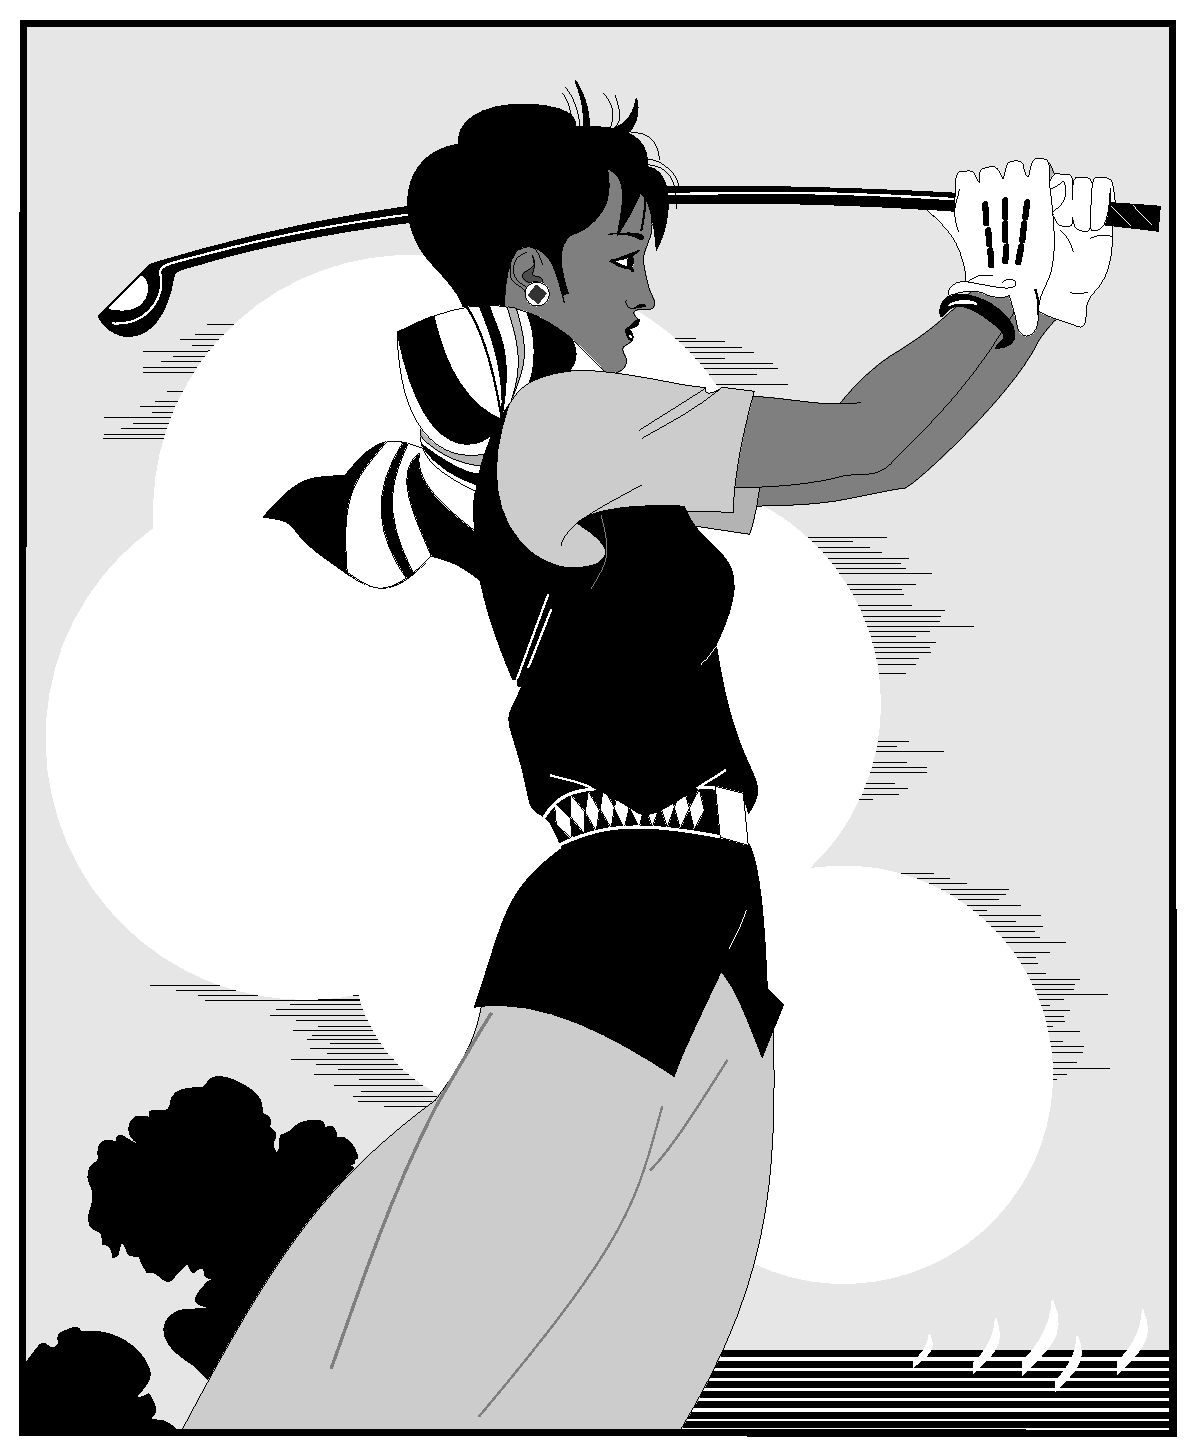
\includegraphics[width=0.2\textwidth]{golfer}}
			\fbox{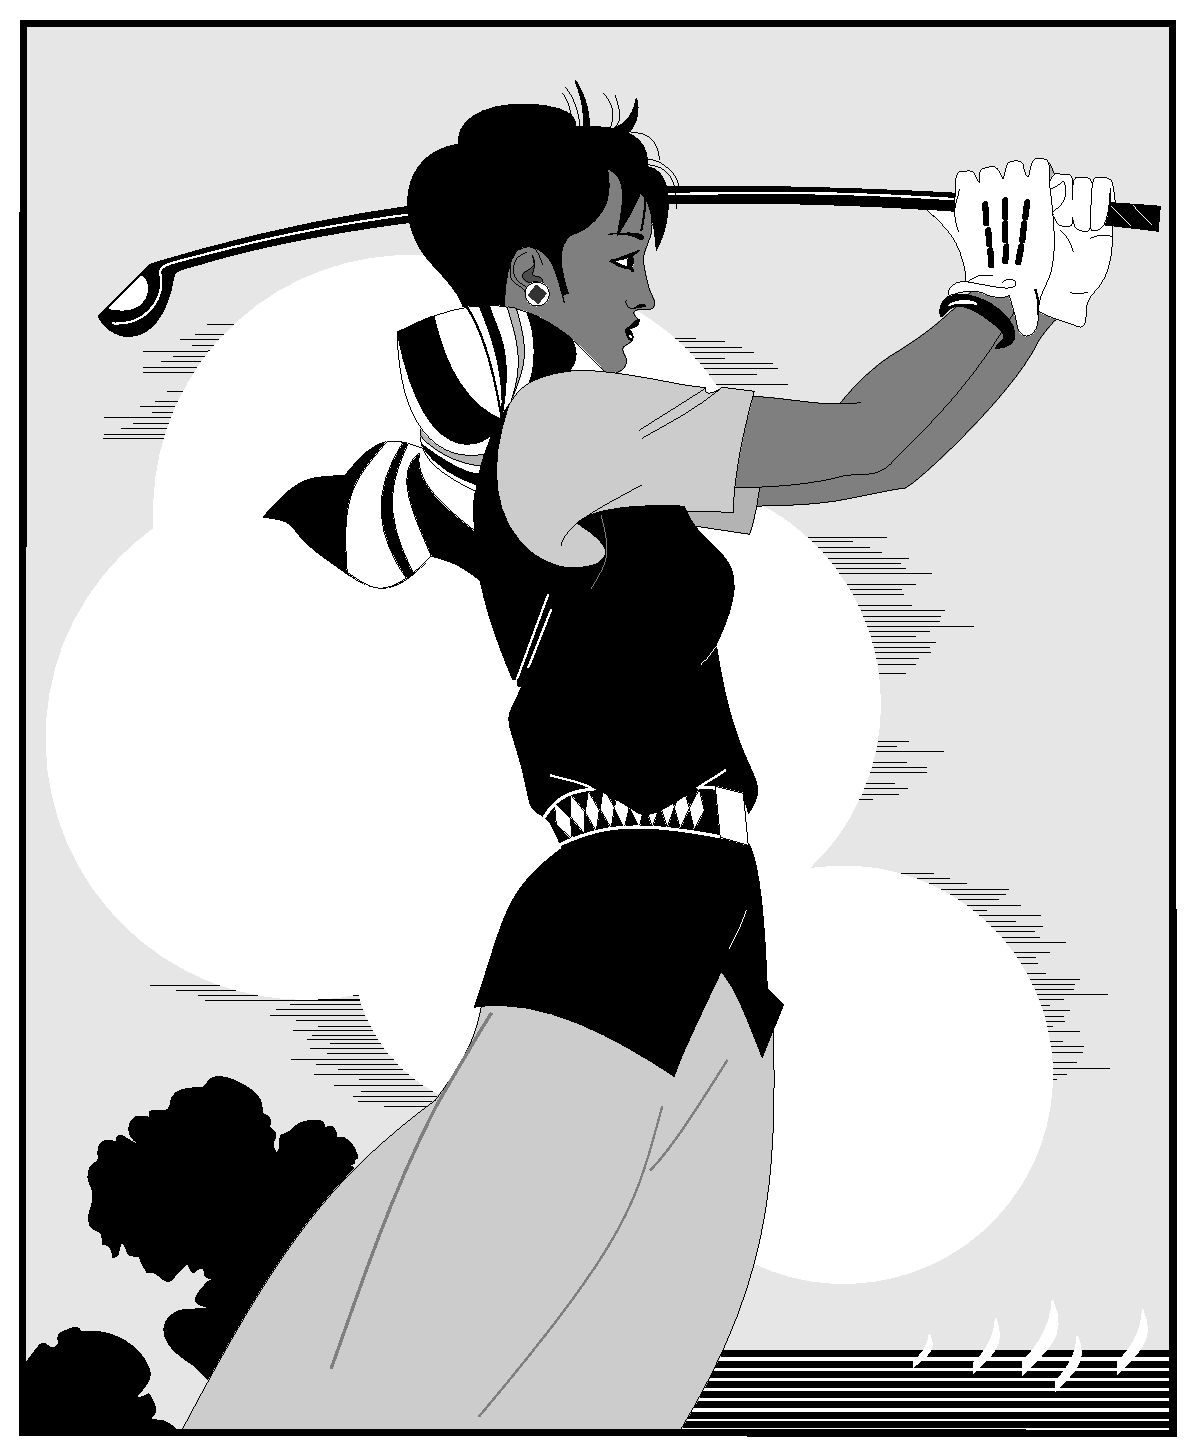
\includegraphics[width=0.2\textwidth]{golfer}}
			\fbox{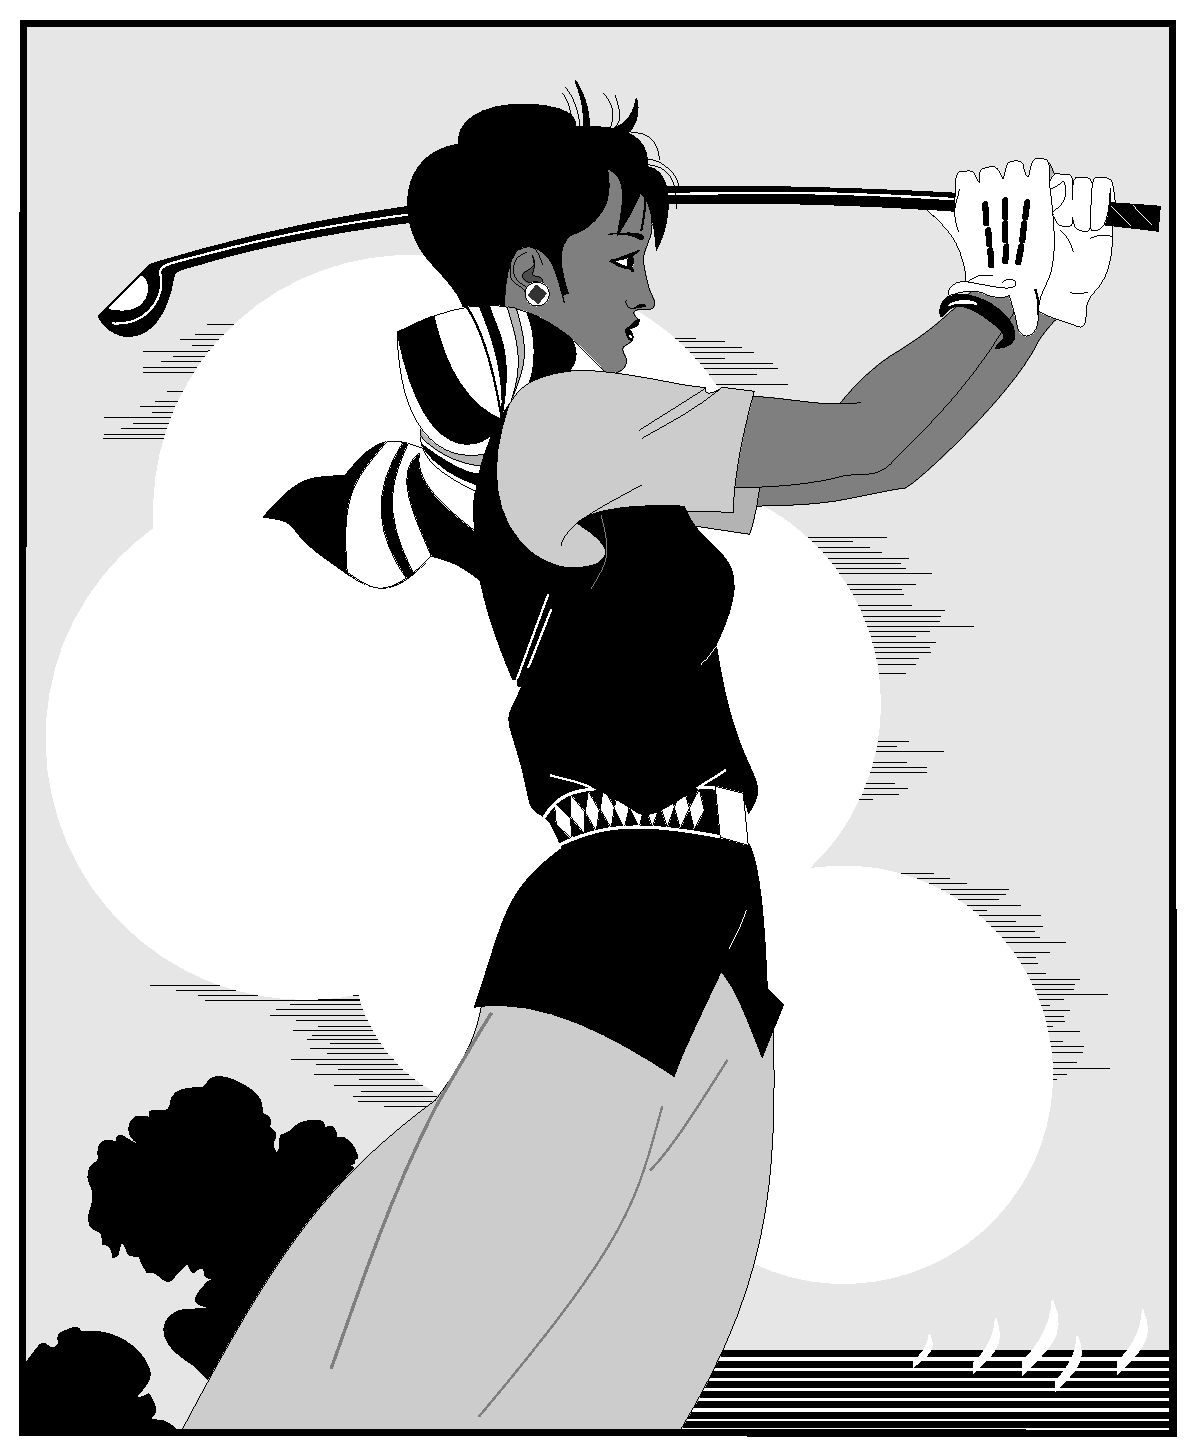
\includegraphics[width=0.2\textwidth]{golfer}}
			\fbox{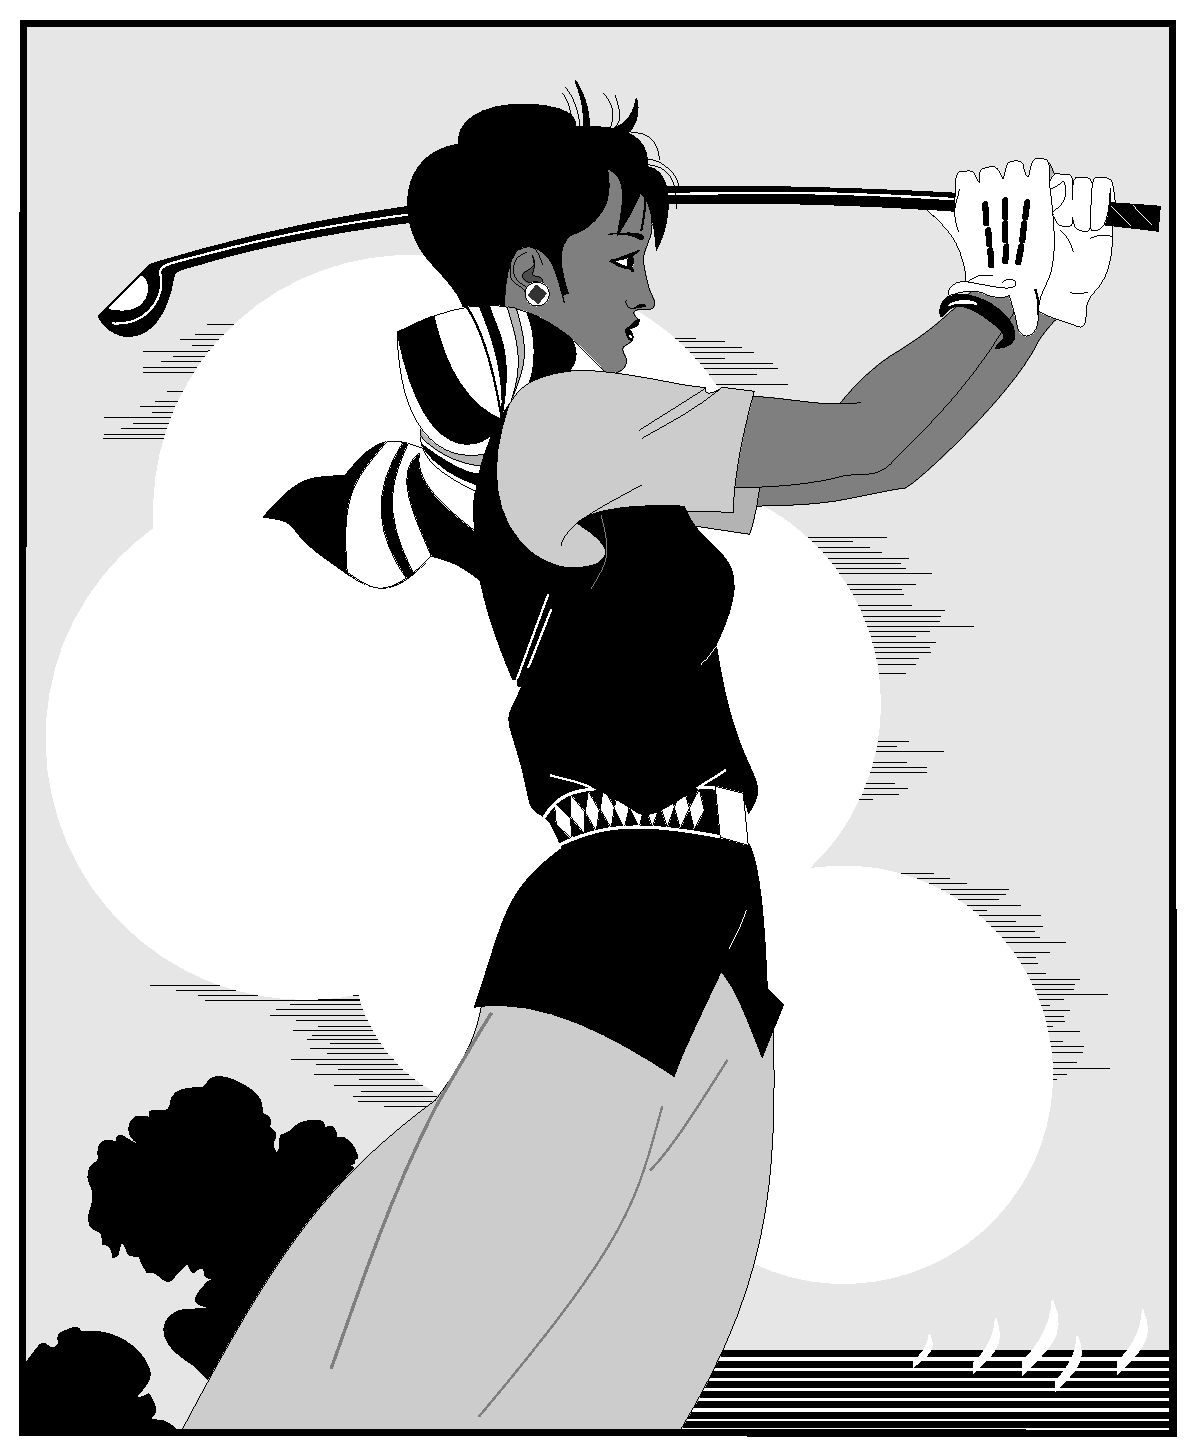
\includegraphics[width=0.2\textwidth]{golfer}}
\bicaption[golfer7]{}{打高尔夫球的人(非规范要求)}{Fig.$\!$}{The person playing golf (Not stated in the regulation)}
		\end{minipage}
	\end{sideways}
\end{figure}

\clearpage

如果不想让图片浮动到下一章节,那么在此处使用\cs{clearpage}命令。

\section{如何做出符合规范的漂亮的图}

关于作图工具在后文\ref{drawtool}中给出一些作图工具的介绍,此处不多言。
此处以R语言和Tikz为例说明如何做出符合规范的图。

\subsection{Tikz作图}

使用Tikz作图核心思想是把格式、主题、样式与内容分离,定义在全局中。
注意字体设置可以有两种选择,如果字少,用五号字,字多用小五。
使用Tikz作图不会出现字体问题,字体会自动与正文一致。

\subsection{R作图}

R是一种极具有代表性的典型的作图工具,应用广泛。
与Tikz图不同,R作图分两种情况:(1)可以转换为Tikz码;(2)不可转换为Tikz码。
第一种情况图形简单,图形中不含有很多数据点,使用R语言中的Tikz包即可。
第二种情况是图形复杂,含有海量数据点,这时候不要转成Tikz矢量图,这会使得论文体积巨大。
推荐使用pdf或png非矢量图形。
使用非矢量图形时要注意选择好字号(五号或小五),和字体(宋体、新罗马)然后选择生成图形大小,注意此时在正文中使用\cs{includegraphics}命令导入时,不要像导入矢量图那样控制图形大小,使用图形的原本的
宽度和高度,这样就确保了非矢量图形中的文字与正文一致了。

为了控制\hitszthesis\ 的大小,此处不给出具体举例。

\subsection{专业绘图工具}[Processional drawing tool]
\label{drawtool}

推荐使用tikz包,使用tikz源码绘图的好处是,图片中的字体与正文中的字体一致。具体如
何使用tikz绘图不属于模板范畴。

tikz适合用来画不需要大量实验数据支撑示意图。但R语言等专业绘图工具具有画出各种、
专业、复杂的数据图。R语言中有tikz包,能自动生成tikz码,这样tikz几乎无所不能。
对于排版有极致追求的小伙伴,可以参考
\href{http://www.texample.net/tikz/resources/}{http://www.texample.net/tikz/resources/}
中所列工具,几乎所有作图软件所作的图形都可转成tikz,然后可以自由的在tikz中修改
图中内容,定义字体等等。实现前文窝工规范中要求的图中字体的一致性的终极目标。

\lipsum[1]

\section{本章小结}[Brief summary]

\lipsum[1]
